\documentclass{sagej}

\runninghead{Short-term orbital effects of radiation pressure on the Lunar Reconnaissance Orbiter}
\title{Short-term orbital effects of radiation pressure \\ on the Lunar Reconnaissance Orbiter}
\author{Dominik Stiller, Dominic Dirkx}
\affiliation{Faculty of Aerospace Engineering, Delft University of Technology, The Netherlands}
% \email{dstiller@uw.edu}
\keywords{Radiation pressure, Lunar Reconnaissance Orbiter, precision orbit determination, force modeling}


\makeglossaries
\newacronym{lro}{LRO}{Lunar Reconnaissance Orbiter}



\begin{abstract}
    Precision orbit determination for geodetic applications requires force models even for small perturbations. Radiation from the Sun and Moon is a significant source of perturbation in lunar orbits and inadequate modeling of \gls{RP} can lead to large position errors. This paper describes the short-term effect of \gls{RP} on the \gls{LRO}, which has a position knowledge requirement of 50 m to 100 m in total and below 1 m radially. We compared models of varying complexity to determine the benefits and computational cost of high-accuracy \gls{RP} modeling. We found that
    \begin{enumerate*}[label=(\arabic*)]
        \item the accelerations differ greatly depending on the Sun position,
        \item only a paneled spacecraft model can account properly for changing orientation and geometry of \gls{LRO}, and
        \item a constant-albedo model is sufficient for lunar radiation, which is dominated by the thermal component. A spherical harmonics model for lunar albedo increases computational cost with little gain in the attained accuracy.
    \end{enumerate*}
    If \gls{RP} is neglected, the along-track position errors can be as large as 1100 m and the radial error varies periodically with an amplitude of up to 24 m, highlighting the importance of adequate force modeling to meet LRO's orbit determination requirements.
\end{abstract}




\begin{document}


\maketitle

\printacronyms[style=inline,title={Abbreviations}]



\section{Introduction}
\label{sec:introduction}

Precision orbit determination is a cornerstone of satellite navigation and spaceborne geodesy. Only if the state, and particularly the position, of the spacecraft are known accurately can the high precision of modern instruments for gravity field recovery or satellite altimetry be exploited fully. Next to tracking data, force models accounting for gravity, solid tides, drag, and other accelerations have the largest role in improving orbit determination. Another important non-conservative force is \acrfull{RP}, which can have magnitudes similar to third-body and irregular gravity field perturbations~\cite{Montenbruck2000}. \gls{RP} arises from the exchange of momentum between electromagnetic radiation and the spacecraft. Neglecting or mismodeling \gls{RP} accelerations can deteriorate position knowledge below acceptable levels.

The \acrfull{LRO} was launched in June 2009 to identify safe landing sites, locate resources, and characterize the radiation environment for future human missions to the Moon~\cite{Tooley2010}. To fulfill these objectives, \gls{LRO} is equipped with instruments to, among other objectives, create high-resolution maps of the lunar topography and gravity field. Accuracies of \qtyrange{50}{100}{\m} in the total position and sub-meter accuracy in the radial component are required to take advantage of the instrument resolutions~\cite{Chin2007,Zuber2009}, which necessitates force models even for small perturbations. Solar \gls{RP} \enquote{is the largest non-gravitational perturbation affecting the LRO orbit and inadequate modeling [\ldots] is the primary cause of large prediction errors for LRO, particularly during high-beta angle periods}~\cite{Slojkowski2015}. The Moon itself is also a significant radiation source since there is no atmosphere and especially the lunar highlands are reflective~\cite{Floberghagen1999}. The orbit determination error is also highly dependent on the modeling of how \gls{RP} translates to accelerations; particularly during full-Sun periods, a model accounting for \gls{LRO}'s geometry and the real orientation of the solar array and high gain antenna outperforms a simple spherical model~\cite{Slojkowski2014}.
 
This paper describes the short-term effects of \gls{RP} on \gls{LRO}'s orbit and the sensitivities of these effects to models of varying complexity. Other authors have already described their orbit determination approaches for \gls{LRO}~\cite{Mazarico2011,Mazarico2018,Nicholson2010,Smith2008,Slojkowski2014,Slojkowski2015,Bauer2016,Maier2016}, but none compared \gls{RP} modeling choices and their implications. \citeauthor{Vielberg2020} investigated the effect of different models for Earth~\cite{Vielberg2020}, where a plethora of observations are available and the radiation environment differs greatly from the Moon. Therefore, their results do not apply to orbits around the Moon. Our paper alleviates this lack of guidance for lunar orbits by elucidating the choice of force models for orbit determination both in terms of accuracy and computational performance. The results relate to short-term effects over 2.5 days, which is a typical arc used in orbit determination. Long-term effects, which may cancel or compound over the span of months, are not considered here.

The \gls{Tudat} was used for all orbital simulations and the models presented here were integrated into the software, which is freely available at \url{https://docs.tudat.space/}.

{\let\thefootnote\relax\footnotetext{\sagesf Email: dstiller@uw.edu}}

\section{Radiation pressure modeling}
\gls{RP} modeling needs to consider the causes and effects of radiation. This section presents a range of cooperating models for both that can be flexibly composed.


\subsection{Mechanics of radiation pressure}
\label{subsec:general-rp-mechanics}

\gls{RP} results from the momentum transfer between electromagnetic radiation and a surface. A spacecraft may receive such radiation from the Sun but also from other celestial bodies: planets and moons emit albedo radiation through reflection of sunlight and thermal radiation depending on surface temperature. The \gls{RP} exerts a force on the spacecraft governed by surface properties such as area, reflectivity and absorptivity. The resulting acceleration is the result of a complex interplay of the bodies emitting radiation (the ``sources'') and the spacecraft receiving the radiation (the ``target'').

Radiation can characterized by the radiant flux density, which commonly has units of \unit{\irr}. Radiosity is the \emph{emitted and reflected} radiant flux density of an opaque surface. The irradiance $E$ is the \emph{incident} radiant flux density on a surface and provides a convenient way to decouple source and target models: the irradiance and the direction of incidence are sufficient to determine the target acceleration, independent of the actual source. We can combine this information into a vector quantity which we call directional irradiance $\vb E = E \vu r_{t/s}$, where $\vu r_{t/s}$ is the unit vector in the source-to-target direction. One or more directional irradiances, which can be though of as light rays, are the output of a source model and used as input to the target model. The \gls{RP} exerted on an irradiated surface is proportional to $1/c$, where $c = \qty{299792458}{m/s}$ is the speed of light. Given the magnitude of $c$, \gls{RP} is usually small (around \qty{4.5e-6}{\N\per\m\squared} for solar radiation at Earth, where $E=\qty{1361}{\irr}$~\cite{Kopp2011}).

Electromagnetic radiation is often composed not just of a single wavelength but rather a range of wavelengths. The distribution can be described by the spectral irradiance in units of \unit{\W\per\square\m\per\Hz}. Since surface properties are often wavelength-dependent, the target model would also have to be aware of the distribution. However, the surface properties as a function of wavelength are often not known, which is also the case for \gls{LRO}. Therefore, we assume the irradiance from source models to be integrated over the whole spectrum and the surface properties of the target model to be valid for all wavelengths.




\subsection{Reflectance distribution}
\label{subsec:general-reflectance-distribution}

Describing the reflectance of a surface is key to \gls{RP} modeling. Both the way a source reflects sunlight and the direction a target is accelerated in depend on the angular distribution of reflectance.

\subsubsection{General reflectance distribution}
In general, reflectance comprises a diffuse (scattered in many directions) and a specular (mirror-like) component. The remaining energy is absorbed by the surface. The reflectance varies with surface normal $\vb N$, incoming radiation direction $\vb L$, and observer direction $\vb V$. This geometry is shown in \cref{fig:reflection-geometry}. A \gls{BRDF} describes the fraction of irradiance reflected towards the observer per steradian, i.e.~\cite{Wetterer2014}
\begin{align}
    f_r (\theta_i, \phi_i, \theta_r, \phi_r)
    = \frac{dL_r(\theta_r, \phi_r)}
    {dE_j(\theta_i, \phi_i)},
\end{align}
where $dL_r$ is the reflected radiance (the directional counterpart to radiosity, typically in \unit{\W\per\square\m\per\steradian}) and $dE_j$ is the received irradiance.

% TODO expand figure with diffuse and specular reflection (e.g. Montenbruck 2000, p. 85)

\begin{figure}[t]
    \centering
    \includegraphics[width=0.8\linewidth]{figures/reflection_geometry.ai}
    \caption{Geometry of a \gls{BRDF} for a surface with normal $\vb N$, incoming direction $\vb L$, and observer direction $\vb V$. The viewing angle $\theta_r$ is between $\vb N$ and $\vb V$. The phase angle (not labeled) is between $\vb L$ and $\vb V$. Adapted from~\cite{Wetterer2014}.}
    \label{fig:reflection-geometry}
\end{figure}

The planetary surface \gls{BRDF} directly leads to the albedo irradiance received by a target if the sun irradiance at the planet surface and the solid angle subtended by the target are known.

The target surface \gls{BRDF} gives the direction in which the target is accelerated through integration over all directions $\vb V$ in which radiation is reflected. The unitless reaction vector, which includes both the direction and magnitude based on absorped, specularly and diffusely reflected fractions, is therefore~\cite{Wetterer2014}
\begin{align}
    \label{eq:brdf-reaction-general}
    \vb R = -\left[ \vb L + \int_{0}^{2\pi} \int_{0}^{\pi/2} f_r \cos\theta_r \vb V d\theta_r d\phi_r \right].
\end{align}
This vector encapsulates the mechanics of momentum transfer. The reaction is minimal for pure absorption ($f_r = 0$). The reaction is maximal (double the minimum) for pure specular reflection in the incidence direction.

\subsubsection{Specular--diffuse reflectance distribution}
A simplified \gls{BRDF} is usually more practical for \gls{RP} modeling: the reflectance is assumed to be a mix of an ideal Lambertian diffuse component and a purely mirror-like specular components. Such a \gls{BRDF} is given by~\cite{Wetterer2014}
\begin{align}
    \label{eq:brdf-specular-diffuse}
    f_r = C_d \frac{1}{\pi} + C_s \frac{\delta(\vb V - \vb M)}{\cos \theta_i}
\end{align}
where $C_d$ and $C_s$ are the diffuse and specular reflectivity coefficients. Together with the absorption coefficient $C_a$, energy is conserved when $C_a + C_d + C_s = 1$. The vector $\vb M = 2\cos\theta_i\vb N - \vb L$ is the direction of $\vb L$'s mirror-like reflection, which only contributes if $\vb V = \vb M$.

For this simplified \gls{BRDF}, the integral in \cref{eq:brdf-reaction-general} evaluates analytically to~\cite{Montenbruck2014}
\begin{align}
    \label{eq:brdf-reaction-specular-diffuse}
    \vb R = - \left[ (C_a + C_d) \vb L + \frac{2}{3} C_d \vb N + 2 \cos\theta_i C_s \vb N \right].
\end{align}
If the target is in thermodynamic equilibrium, all absorbed radiation is reradiated instantaneously by Kirchhoff's law. If this reradiation is Lambertian, the reaction vector becomes~\cite{Montenbruck2014}
\begin{align}
    \label{eq:brdf-reaction-specular-diffuse-instrerad}
    \vb R = - \left[ (C_a + C_d) \left(\vb L + \frac{2}{3} \vb N\right) + 2 \cos\theta_i C_s \vb N \right].
\end{align}
The specular contribution is strictly along the surface normal direction since its tangential components cancel. The Lambertian diffuse contribution (both reflected and reradiated) has a component along the incoming direction but also, weighted by a factor $2/3$ (see~\cite{Ziebart2004} for a derivation of this factor), a component along the surface normal. The reaction vector is thus always in the plane spanned by $\vb L$ and $\vb N$.



\subsection{Radiation sources}
\label{subsec:radiation-sources}

Radiation sources emit or reflect radiation, which exerts \gls{RP} onto the target. As explained in \cref{subsec:general-rp-mechanics}, the incident radiation at a target due to a source can be thought of as light rays, which are described by their directional irradiance at the target. How the directional irradiance is calculated depends on the type of source.

\subsubsection{Isotropic point sources}
The simplest source model is a point source that isotropically radiates in all directions. This model is appropriate for far-away sources such as the Sun at \qty{1}{\astronomicalunit} distance. Due to the distance, all rays are effectively parallel and can be merged into a single ray parallel to the source-to-target vector $\vb r_{t/s}$. For an isotropic source, the total luminosity $L$ (units of \unit{\W}) is uniformly distributed over a sphere, leading to an inverse square law. Therefore, the irradiance at the target is
\begin{align}
    \label{eq:irradiance-point-luminosity}
    E = \frac{L}{4\pi\norm{\vb r_{t/s}}^2}.
\end{align}
Alternatively, a reference irradiance $E_\textnormal{ref}$ observed at a distance $\vb r_\textnormal{ref}$ can be scaled:
\begin{align}
    E = E_\textnormal{ref} \frac{r_\textnormal{ref}}{\norm{\vb r_{t/s}}^2}.
\end{align}
The solar luminosity is \qty{3.828e26}{\W}~\cite{Prsa2016}, which corresponds to an irradiance of \qty{1361}{\irr} at \qty{1}{\astronomicalunit}. Note that these values are averages, which vary with the 11-year solar cycle by about \qty{0.1}{\percent} and more on shorter timescales due to sunspot darkening and facular brightening~\cite{Kopp2016}. Observational time series exist to account for these variations~\cite{Dewitte2017}.

\subsubsection{Paneled sources: Discretization}
Radiation due to planets and moons requires more involved source models. Planetary emissions comprise reflected solar radiation and thermal infrared radiation~\cite{Knocke1988}. The fraction of reflected sunlight is called albedo\footnote{Two types of albedo exist: spherical/Bond albedo is the fraction of sunlight reflected in all directions, while geometrical albedo is the fraction of sunlight reflected with respect to an ideal diffuse surface for normal incidence and viewing directions~\cite{Heiken1991}. For our purpose, spherical albedo is appropriate and synonymous with albedo in this paper.} $a$; the corresponding type is therefore also called albedo radiation. Thermal radiation is due to absorbed solar energy that is re-emitted in a delayed fashion. Observation time series of albedo and thermal fluxes exist for Earth~\cite{Dewitte2017}, but physical modeling is required for the Moon.

Since planetary radiation is not isotropic and the spacecraft is typically much closer to the body than to the Sun, the source extent has to be considered. In contrast to the previously described point source, we therefore model Earth and Moon as extended sources. These are discretized into sub-sources, from which rays emanate that are, in general, not parallel. The sub-sources can be thought of as panels with an area, orientation, position, and radiosity model. The panel extent is represented by the area but any other panel properties are only evaluated at its center. A panel only radiates from the positive normal side, not from the backside.

Different algorithms exist to divide the planet ellipsoid into panels. Some authors use a longitude--latitude grid (e.g.,~\cite{RodriguezSolano2011a,Woeske2019}, particularly with observed fluxes) or generate static, uniformly spaced panels over the whole sphere (e.g.,~\cite{Wetterer2014}). However, both approaches are inefficient for low-altitude spacecraft, which require a large number of panels, most of which are never visible. Therefore, the de-facto standard is the dynamic\footnote{Dynamic refers to the fact that panels move with the spacecraft, as opposed to static paneling, for which panels are invariant with spacecraft position or time.} paneling method introduced by \citeauthor{Knocke1988}~\cite{Knocke1988}.

% TODO expand: describe Knocke paneling in detail, with figure for zeta, beta...

In Knocke's method, only the visible area of the planet is paneled. This area is a spherical cap, centered at the subsatellite point and divided into concentric rings that are, again, divided into equal-area segments. A central panel is located at the subsatellite point. All panels contribute to the irradiance received by the target. However, the effective area of each panel is projected by its viewing angle $\theta_r$ (see \cref{fig:reflection-geometry}) and the irradiance is attenuated by an inverse square law. In Knocke's method, the rings are spaced such that each panel has the same projected, attenuated area. The projected, attenuated area of a panel is defined as~\cite{Knocke1988}
\begin{align}
    \frac{\dd{A} \cos \theta_r}{\norm{\vb r_{t/s}}^2},
\end{align}
where $\dd{A}$ is the geometric panel area and $r_{t/s}$ is the source-to-target vector (in this case, the panel-to-target vector). More rings and more panels per ring improve the fidelity of the calculated irradiance, barring the resolution limit of the radiosity model (e.g., the albedo distribution). While arbitrary numbers of panels per ring are possible, Knocke suggests multiples of 6 (i.e., six panels in the first ring, twelve panels in the second ring, \dots). The algorithm is elaborated in~\cite{Knocke1989}.

\begin{figure*}[t]
    \centering

    \begin{subfigure}[c]{0.49\textwidth}
        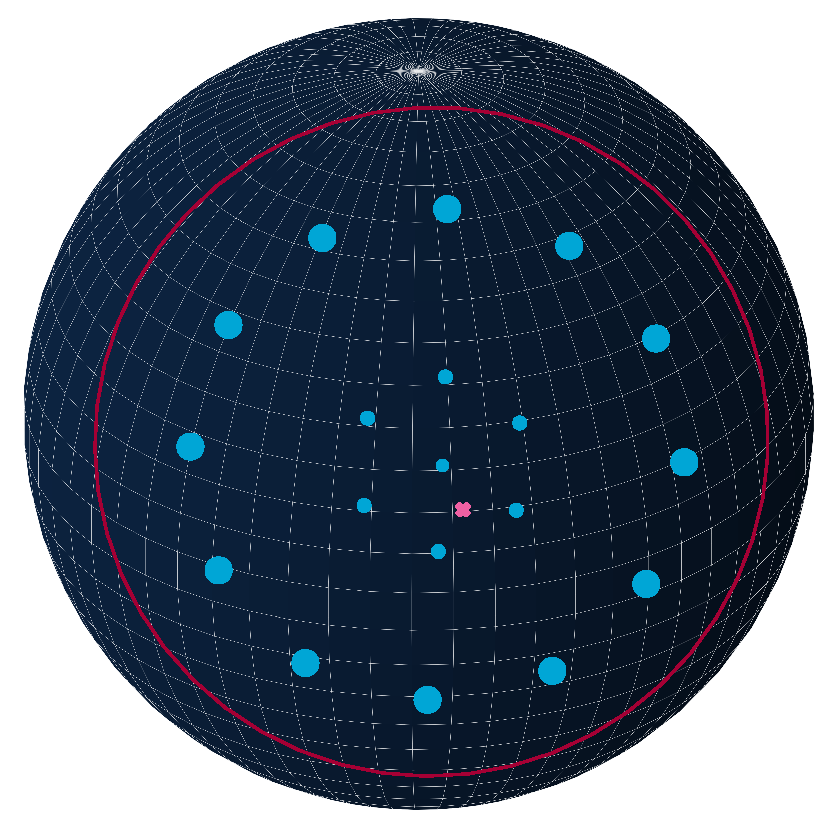
\includegraphics[width=\textwidth]{figures/plots/knocke_paneling_high.pdf}
        \subcaption{High altitude: $h = \qty{1500}{\km}$, 2 rings, angular diameter of cap = \ang{115}.}
    \end{subfigure}
   \hfill
    \begin{subfigure}[c]{0.49\textwidth}
        
\includegraphics[width=\textwidth]{figures/plots/knocke_paneling_low.pdf}
        \subcaption{Low altitude: $h = \qty{50}{\km}$, 6 rings, angular diameter of cap = \ang{27}.}
        \label{fig:general-knocke-paneling-low}
    \end{subfigure}

   \caption{Panels generated with Knocke's algorithm for the Moon, which has a polar radius of \qty{1737}{\km}. The spacecraft (\textcolor{mpl-pink}{\ding{54}}) sees a spherical cap (\textcolor{mpl-red}{\textbf{---}}), which contains rings of panels and is larger at higher altitudes $h$. Panel centers (\textcolor{mpl-lightblue}{\ding{108}}) are scaled proportional to the panel area. The panels have equal projected, attenuated areas and are therefore concentrated around the subsatellite point. The scenario in \protect\subref{fig:general-knocke-paneling-low} corresponds to LRO's orbit and the paneling used in this paper.}
   \label{fig:general-knocke-paneling}
\end{figure*}

Two examples at different spacecraft altitudes and with different ring numbers are shown in \cref{fig:general-knocke-paneling}. At higher altitudes, a larger area is visible (approaching a hemisphere) and panels are somewhat more uniform in area. At lower altitudes, the panels are more tightly spaced towards the subsatellite point. In both cases, panel areas increase towards the edge of the visible cap. This pattern is result of the equal projected, attenuated areas.

\subsubsection{Paneled sources: Radiosity models}
The emitted and reflected fluxes of a panel are described by a radiosity model. The irradiance at the target position can then be derived from the panel radiosity. Both radiosity and irradiance commonly have units of \unit{\irr}. Each panel can have one or more radiosity model, usually one for albedo radiation and one for thermal radiation. We present three such models.

The albedo radiosity model accounts for diffuse Lambertian reflection of solar radiation. It implements the specular--diffuse \gls{BRDF} from \cref{eq:brdf-specular-diffuse} with $C_s = 0$ and the albedo value $C_d = a$ at the panel center. The albedo radiosity of a panel is~\cite{Knocke1988}
\begin{align}
    \label{eq:radiosity-albedo}
    J_\textnormal{albedo} = a \left(\cos\theta_i\right)_+ E_s,
\end{align}
where $E_s$ is the incoming solar irradiance at the panel (e.g., as found from \cref{eq:irradiance-point-luminosity}) and the solar incidence angle $\theta_i$ is defined in \cref{fig:reflection-geometry}. The operator $(\cdot)_+$ restricts the input to positive values or zero otherwise. This ensures that no radiation is reflected from the backside.

The delayed thermal radiosity model assumes that absorbed radiation is emitted independently of incident solar radiation and the radiosity is thus not a function of $\theta_i$. The only spatial variations arise from emissivity differences. The emissivity $e$ of a surface is the ratio of the actual radiosity to the ideal black body radiosity. The delay arises from the planet's large thermal inertia. The delayed thermal radiosity of a panel is~\cite{Knocke1988}
\begin{align}
    \label{eq:radiosity-thermal-delayed}
    J_\textnormal{thermal} = e \frac{E_s}{4},
\end{align}
where $e$ is the emissivity of the panel, evaluated at its center. The factor 1/4 is the ratio of absorbing area (a circle) to emitting area (a sphere). The albedo and delayed thermal model were originally used by \citeauthor{Knocke1988} for Earth emissions~\cite{Knocke1988}.

The angle-based thermal radiosity model is more appropriate than the delayed model if the surface experience significant diurnal cooling and heating. The surface temperature is modeled as a function of the solar incidence angle $\theta_i$ and related to the radiosity through the Stefan--Boltzmann law. The surface temperature is interpolated between the minimum and maximum temperatures, $T_\textnormal{min}$ and $T_\textnormal{max}$ as
\begin{align}
    \label{eq:surface-temperature}
    T = \max\left( T_\textnormal{max} \left(\cos\theta_i\right)_+^{1/4}, T_\textnormal{min} \right).
\end{align}
These temperatures typically correspond to the nighttime temperature and the temperature at the subsolar point. The angle-based thermal radiosity of a panel is then~\cite{Lemoine2013}
\begin{align}
    \label{eq:radiosity-thermal-anglebased}
    J_\textnormal{thermal} = e \sigma T^4,
\end{align}
where $T$ is the surface temperature from \cref{eq:surface-temperature} at the panel center and $\sigma = \qty{5.670e-8}{\W\per\m\squared\per\K\tothe{4}}$ is the Stefan--Boltzmann constant. On the dayside, the radiosity is proportional to $T_\textnormal{max}^4\cos\theta_i$. The maximum radiosity of $e \sigma T_\textnormal{max}^4$ is usually larger than the near-constant $e E_s/4$ from \cref{eq:radiosity-thermal-delayed}, but quickly decreases as the panel moves away from the subsolar point (where $\theta_i = \ang{0}$). On the nightside, the thermal radiosity reduces to $e \sigma T_\textnormal{min}^4$.

The albedo and thermal radiosity models depend on the distribution of $a$ and $e$ over the planetary surface. The values may be assumed constant but generally vary with longitude, latitude, and time. Particularly for Earth, seasons and weather greatly affect reflectivity and emissivity~\cite{Goode2001}. Since the Moon lacks seasons, distributions that only vary spatially are appropriate.

To obtain the irradiance at the target due to the panel radiosity, we assume that the emission follows Lambert's cosine law and account for the projected, attenuated area of the source panel. The irradiance therefore is
\begin{align}
    \label{eq:irradiance-from-radiosity}
    E = \left(\sum_{J_i \in \mathcal{J}} J_i\right) \frac{\dd{A} \left(\cos\theta_r\right)_+}{\pi\norm{\vb r_{t/s}}^2},
\end{align}
where $\mathcal{J}$ is the set of radiosities from any of the previous radiosity models. Usually, a panel has the albedo model and one thermal model. Here, the source-to-target vector $\vb r_{t/s}$ uses the panel center position, not the source body center. The direction $\vu r_{t/s}$ of the corresponding directional irradiance $\vb E = E \vu r_{t/s}$  is therefore not the same for each panel and thus considers the extent of the source. The radiosities $J_i$ in \cref{eq:irradiance-from-radiosity} can be summed since their radiation emanates from the same point, the panel center. Contrarily, the directional irradiances $\vb E$ can generally not be summed since the their  individual directions need to be retained: the reflectance model of the target may be sensitive to the incoming direction of each ray. Therefore, a set of directional radiances $\mathcal{E}$ is handed to the \gls{RP} target model for acceleration calculations.




\subsection{Radiation pressure targets}
\label{subsec:radiation-pressure-targets}

A \gls{RP} target is a body that is accelerated by \gls{RP}. The target model governs how the incident irradiances from point sources and extended sources accelerate the target body.


\subsubsection{Cannonball target}
In its simplest form, a target can be modeled as isotropic sphere, also referred to as cannonball. This sphere is characterized by a cross-sectional area $A_c$ (independent of orientation), radiation pressure coefficient $C_r$ (incorporating reflectivity and absorption coefficients), and mass $m$. Due to its isotropy, any lateral components cancel and the net acceleration is always along the source-to-target vector. The \gls{RP} acceleration of a cannonball target is~\cite{Montenbruck2000}
\begin{align}
    \label{eq:cannonball-target}
    \vb a = C_r \frac{A_c}{m}\sum_{\vb E_j \in \mathcal{E}}\frac{\vb E_j}{c},
\end{align}
where the sum is vectorial and $\sum\vb E_j/c$ is the total \gls{RP} as described in \cref{subsec:general-rp-mechanics}. $\mathcal{E}$ is the set of directional irradiances from any number of sources, both point (\cref{eq:irradiance-point-luminosity}) and paneled (\cref{eq:irradiance-from-radiosity}). The dependence on the area-to-mass ratio $A_c/m$ is similar to drag accelerations. While the cannonball model cannot account for complex geometry, it is often used in orbit determination with $C_r$ as estimated variable. Ray tracing of a detailed model can also be used to establish the evolution of $A_c$ and $C_r$~\cite{Hattori2019}.


\subsubsection{Paneled target}
In reality, the cross-section and optical properties of a spacecraft change with orientation and incident direction. This effect is particularly noticeable for solar panels, which are large and usually track the Sun. To account for the geometry and differences in materials, a spacecraft can be represented as a collection of $n$ panels. Each panel is characterized by its area, surface normal, and reflectance distribution. The position would only be relevant for rotational but not for linear accelerations. In case of moving parts, the surface normal may change over time. The reflectance distribution can be given as generic \gls{BRDF}, but is often a specular--diffuse \gls{BRDF}. The \gls{RP} acceleration of a paneled target is~\cite{Marshall1992}
\begin{align}
    \label{eq:paneled-target}
    \vb a = \frac{1}{m} \sum_{\vb E_j \in \mathcal{E}} \left( \frac{\norm{\vb E_j}}{c} \sum_{k=1}^n A_k \left(\cos\theta_{i,k}\right)_+ \vb R_k\right),
\end{align}
where the indices $j$ and $k$ denote the (sub-)source and target panel, respectively. $A_k$ is the area of the $k$-th panel. $\theta_{i,k}$ is the incidence angle of $\vb E_i$ onto the $k$-th panel. $\vb R_k$ is the reaction vector as defined by {\renewcommand\creflastconjunction{ or }\cref{eq:brdf-reaction-general,eq:brdf-reaction-specular-diffuse,eq:brdf-reaction-specular-diffuse-instrerad}}, depending on the \gls{BRDF}. The reaction vector is a function of the panel surface normal $\vb N$ and the source-to-target direction $\vb L = \vu E_j$. Therefore, the inner sum has to be evaluated for each directional irradiance $\vb E_j$ of the outer sum. In general, the resulting acceleration is not along the source-to-target direction as for the cannonball.

Extensions for the paneled target model exist. The model described above does not account for self-shadowing, which is occurs when one ray would intersect two panels. This effectively reduces the area of the shadowed panel, an effect that can be significant for complex spacecraft geometries~\cite{Mazarico2009}. Polygon intersections enable simple calculation of the effective area~\cite{Mazarico2009}. Ray tracing is more involved but can also account for multiple reflections between target panels~\cite{Kenneally2020}.

Another extension is the radiation pressure due to thermal radiation of the spacecraft itself. Instantaneous reradiation as modeled by \cref{eq:brdf-reaction-specular-diffuse-instrerad} for the case of thermodynamic equilibrium is a simple version of this. In reality, panels heat up and cool down (particularly during eclipses) through radiation, conduction, and internal heat production. Advanced models therefore calculate the temperature of each panel. Such models range from a simple heat balance~\cite{Wetterer2014} to finite element models~\cite{Woeske2019}. However, lack of knowledge of the thermal properties may restrict the applicability. For the sake of simplicity, neither self-shadowing nor thermal radiation pressure of the spacecraft is considered in this paper.

% TODO expand add figure how symbols fit together



\subsection{Occultation}
All previous models assume that the line of sight between source and target is unobstructed. However, occultation is a common astronomical phenomenon: a low-altitude spacecraft may be in the planet's shadow for more than a third of its orbit, and partial or full lunar eclipses can occur multiple times per year. We present two occultation models.

\begin{figure}[b]
    \centering
    \includegraphics[width=\linewidth]{figures/eclipse_geometry.ai}
    \caption{Conical occultation model for spherical sources and occulting bodies. The observer is partially illuminated in the penumbra but fully shadowed in the umbra. Adapted from~\cite{Vallado2013}.}
    \label{fig:eclipse-geometry}
\end{figure}

\subsubsection{Shadow function}
The shadow function $\nu$ describes the fraction of light received from a spherical source in the presence of an occulting spherical body. The geometry of the conical occultation model is shown in \cref{fig:eclipse-geometry}. In the umbra, the source is fully occulted and the observer does not receive any radiation ($\nu = 0$), a state referred to as total eclipse. In the penumbra, the observer can see part of the source ($0 < \nu < 1$). Only outside the shadow region does the observer receive the full radiation ($\nu = 1$). In the case of a lunar eclipse, Earth occults the Sun and casts a shadow onto the Moon such that there is no lunar albedo radiation. On the nightside of a planet, the planet itself occults the Sun.

With the models described in \cref{subsec:radiation-sources,subsec:radiation-pressure-targets}, the shadow function needs to be considered for radiation from a point source, both when directly incident on the target and when used as solar radiation for albedo radiosity. The extent of the source and occulting bodies needs to be known for shadow function calculations, even in the case of point sources. A derivation of the conical model for $\nu$ is presented by \citeauthor{Montenbruck2000}~\cite{Montenbruck2000}.

The conical model can only account for one occulting body. In case of multiple occulting bodies, shadows might overlap and the product of their shadow functions would underestimate the actual received fraction. Knowledge of the shadow intersection would be required to avoid this. \citeauthor{Zhang2019} derived a model for two occulting bodies~\cite{Zhang2019}. However, only single occultations are considered in this paper.

More involved shadow models exist that improve prediction of the penumbra passage. These models can consider planetary oblateness and atmospheric effects like absorption, scattering and refraction~\cite{Li2019}. Other models can account for topography by combining a paneled Sun model with a topography map~\cite{Mazarico2018}. These modification usually prolong the penumbra duration.


\subsubsection{Point-to-point visibility}
For source panels represented by their center point, the shadow function becomes binary: either there is a line of sight between the panel center and the target or there is not. Such point-to-point visibility with a spherical occulting body is easily modeled geometrically. A derivation is given by \citeauthor{Vallado2013}~\cite{Vallado2013}. Multiple occultations are supported in this occultation model by the logical conjunction of the individual visibilities.

\section{Radiation pressure modeling for LRO}

\subsection{Lunar albedo radiation}
\label{subsec:lunar-albedo}

\begin{figure*}[t]
    \centering

    \begin{subfigure}[c]{0.49\textwidth}
        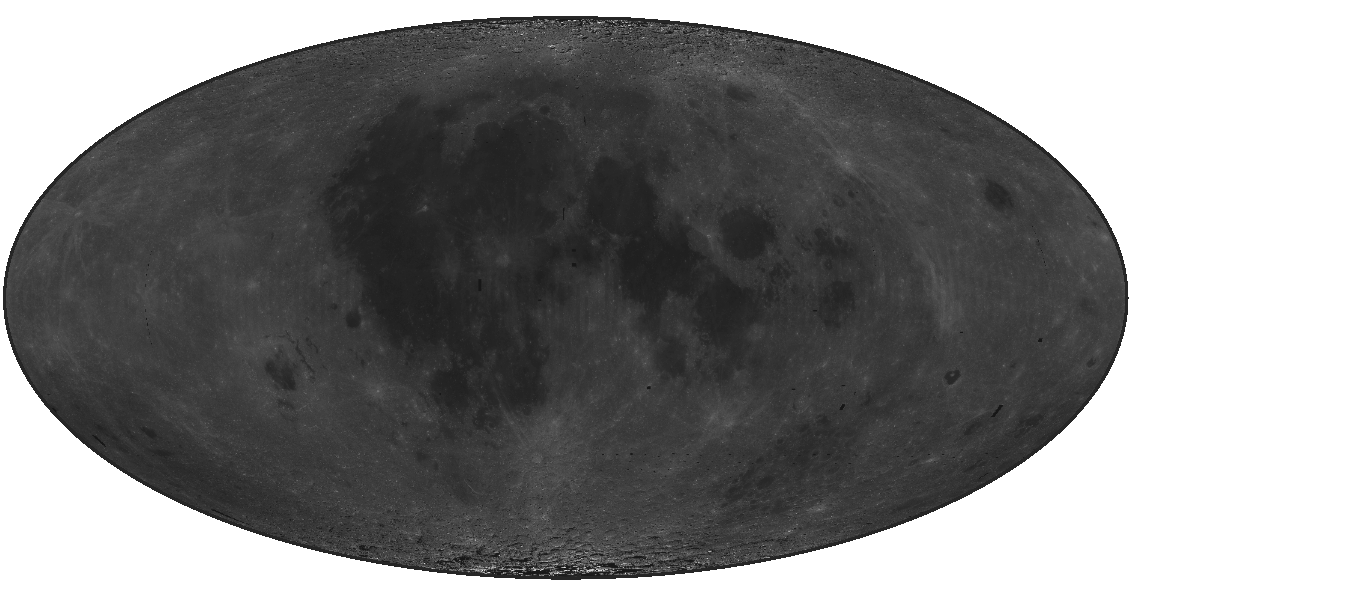
\includegraphics[width=\textwidth]{figures/plots/lunar_map_photo.pdf}
    \end{subfigure}
    \hfill
    \begin{subfigure}[c]{0.49\textwidth}
        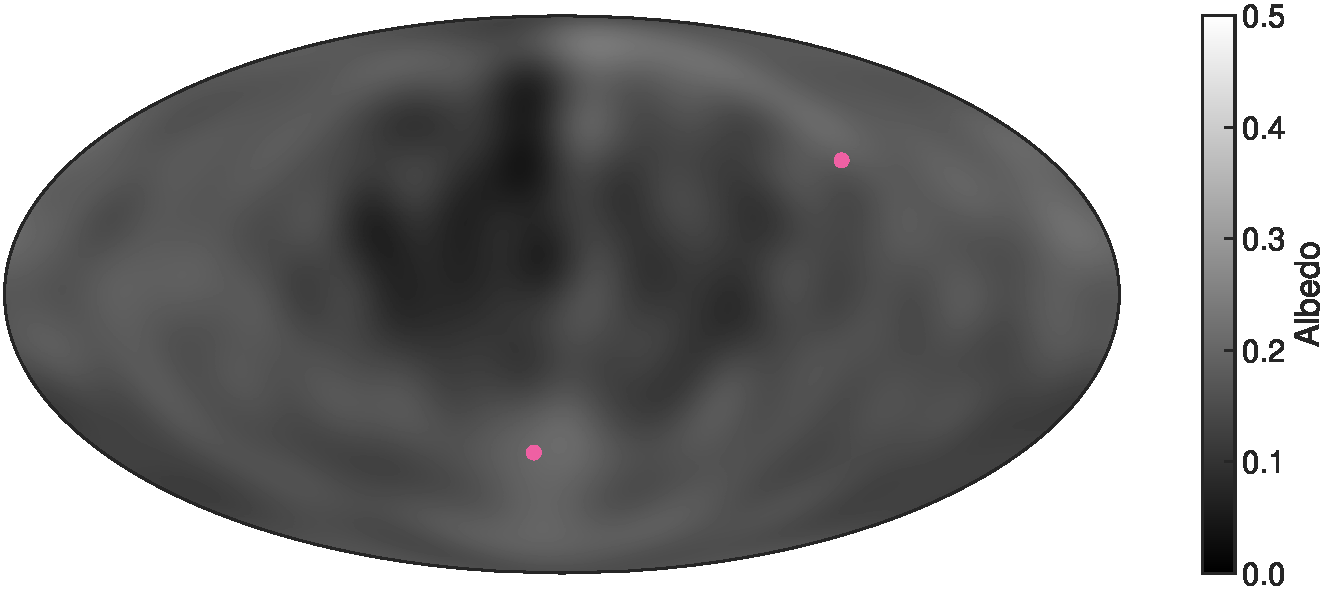
\includegraphics[width=\textwidth]{figures/plots/lunar_map_dlam1.pdf}
    \end{subfigure}
    
    \bigskip
    
    \begin{subfigure}[c]{0.49\textwidth}
        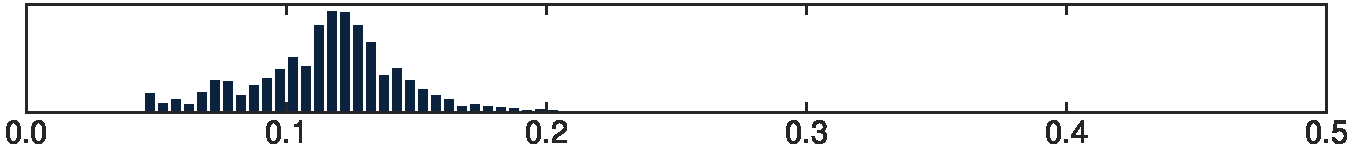
\includegraphics[width=\textwidth]{figures/plots/lunar_hist_photo.pdf}
        \subcaption{Mosaic (mean = 0.12, minimum = 0.05, 99th percentile = 0.29)~\cite{UASC2009}}
        \label{fig:lunar-albedo-map-photo}
    \end{subfigure}
   \hfill
    \begin{subfigure}[c]{0.49\textwidth}
        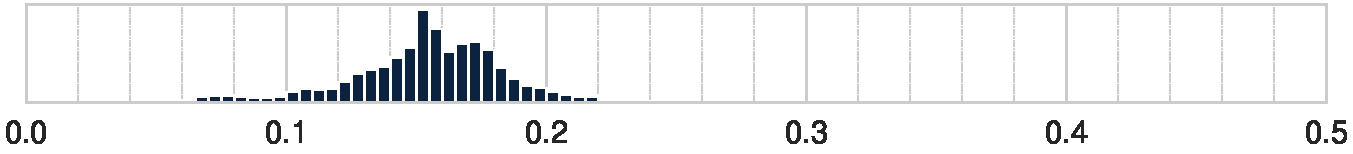
\includegraphics[width=\textwidth]{figures/plots/lunar_hist_dlam1.pdf}
        \subcaption{\acrshort{DLAM1} (mean = 0.15, minimum = 0.04, 99th percentile = 0.22)}
        \label{fig:lunar-albedo-map-dlam1}
    \end{subfigure}

   \caption{Lunar albedo distribution from Clementine. Both the mosaic and \acrshort{DLAM1} are based on 750 nm reflectivity, but \acrshort{DLAM1} has been corrected to the average solar wavelength. Large bright features like the Tycho and Giordano Bruno craters (\textcolor{mpl-pink}{\ding{108}}) can be registered. Note that the maximum of the albedo scale here is 0.5 instead of 1.0 to increase contrast; in reality, the Moon appears half as bright.}
   \label{fig:lunar-albedo-map}
\end{figure*}

The Moon is a major source of radiation in \gls{LRO}'s orbit, with lunar irradiance magnitudes approaching half of the Sun's. Therefore, albedo and thermal radiation due to the Moon will be modeled. While the lunar albedo is only \qty{40}{\percent} of Earth's albedo~\cite{Goode2001}, albedo radiation due to the Moon is still substantial, particularly over the subsolar point~\cite{Floberghagen1999}. Lunar albedo varies significantly with geology: the highlands (mean $a = 0.16$, maximum $a=0.25$) are much more reflective than the maria (mean $a = 0.07$, minimum $a = 0.05$) due to their respective regolith composition~\cite{Vasavada2012,Hayne2017,Sato2014}. The mosaic of calibrated albedo imagery from Clementine in \cref{fig:lunar-albedo-map-photo} clearly shows the differences between highlands and marias. The mean of 0.12 agrees with other literature~\cite{Vasavada2012}, and most of the lunar surface has an albedo below 0.20. Higher values are only found at the poles, where the imagery represents topographic shading rather than actual albedo~\cite{McEwen1997}. Note that the mosaic is for albedo of light at \qty{750}{\nm} wavelength, which is slightly longer than the average solar wavelength. Even though solar radiation has most energy within the \qtyrange{300}{2400}{\nm} band, the spectrum peaks at around \qty{470}{\nm}~\cite{Iqbal1983}. Lunar reflectivity increases with increasing wavelength~\cite{Shkuratov2011}.

\citeauthor{Floberghagen1999}'s \numproduct{15x15} spherical harmonics expansion called \gls{DLAM1}~\cite{Floberghagen1999} is often used to represent this spatial albedo variability in lunar \gls{RP} models. \gls{DLAM1} was fitted from Clementine imagery and was designed to work with Knocke's albedo model for dynamic paneling (\cref{eq:radiosity-albedo}). Due to the nature of spherical harmonics, the model cannot resolve features smaller than \ang{12} (\qty{360}{\km} at the equator). The expansion is shown in \cref{fig:lunar-albedo-map-dlam1}, along with direct imagery from Clementine. \gls{DLAM1} was also derived from 750 nm imagery, but we scale the original values by $1/1.3$ to account for the reduced reflectivity at the average solar solar wavelength. This factor was proposed by \citeauthor{Vasavada2012}~\cite{Vasavada2012}. Even with the correction, the mean albedo of the expansion of 0.15 is still \qty{25}{\percent} above the commonly accepted mean of 0.12. This is possibly due to a different calibration of the imagery that \gls{DLAM1} is based on compared to the mosaic from \cref{fig:lunar-albedo-map-photo}. In fact, Clementine is known to overestimate albedo due to bad calibration~\cite{Shkuratov2011}. Apart from the difference in magnitude, the patterns agree reasonably well: maria and highlands are distinct and large bright features like the ray system around the Tycho and Giordano Bruno craters can be recognized (marked in \cref{fig:lunar-albedo-map-dlam1}).

Despite the shortcomings of \gls{DLAM1}, spherical harmonics are convenient: they are smooth and do not require interpolation like a gridded map. They can easily be truncated to trade detail for computational efficiency. Therefore, we will use \gls{DLAM1} in this paper but consider that the magnitude may be overestimated by \qty{25}{\percent} during the analysis of results. We will also compare results for the location-dependent \gls{DLAM1} with those for a constant value, which should be more computationally efficient. As single representative albedo, we choose the mean of 0.15 instead of 0.12 to facilitate comparison. Note that the spatial variability described above suggests that a single albedo value cannot accurately represent lunar reflectivity.

Albedo radiation assumes ideal, diffuse Lambertian reflectance, which decreases with the cosine of the viewing angle. This assumption is especially appropriate for Earth, for which purely specular radiosity only amounts to \qty{10}{\percent} of the purely diffuse radiosity~\cite{Knocke1988}. However, this is not the case for the Moon: the opposition effect increases the reflectance at low phase angles (when the source is behind the observer, see \cref{fig:eclipse-geometry}) much more than would be expected from a cosine law. In fact, the brightness increases more than \qty{40}{\percent} between phase angles of \ang{4} and \ang{0}~\cite{Buratti1996}. This is primarily caused by shadow hiding. To account for non-diffuse reflectance of the lunar surface, the Hapke \gls{BRDF} was developed~\cite{Hapke2012}. This \gls{BRDF} is an empirical relation based on nine parameters that control, among other phenomena, the strength and directionality of the opposition effect. Near-global maps for these parameters have been fitted from \gls{LRO} observations and could be used for a radiosity model~\cite{Sato2014}. For \gls{RP} acceleration modeling, the opposition effect is only of concern when the target is above the subsolar point; the Sun has to be in the orbital plane for this. For \gls{LRO}, this only occurs for a few days twice a year, and even then only for a small fraction of the orbit. Therefore, we will neglect opposition effect in this study.




\subsection{Lunar thermal radiation}

Lunar surface temperatures and the associated thermal radiation undergoes a significant diurnal cycle. Daytime and nighttime temperatures can differ by up to \qty{290}{\K}. The surface heats rapidly after sunrise, cools at about the same rate after local noon, then slower during the night~\cite{Vasavada2012}. There are small seasonal changes, with the noon temperature differing by \qty{6}{\K} between lunar aphelion and perihelion~\cite{Heiken1991}. The large diurnal variability makes Knocke's delayed thermal model (\cref{eq:radiosity-thermal-delayed}), which gives a constant radiosity throughout the day, unsuitable for the Moon.

Diurnal variability is represented well by the angle-based thermal model (\cref{eq:radiosity-thermal-anglebased}). We parametrize the model with the equatorial temperatures just before sunrise ($T_\textnormal{min} = \qty{95}{\K}$) and at local noon ($T_\textnormal{max} = \qty{385}{\K}$). The model transitions to the nighttime temperature when the incidence angle $\theta_i \geq \ang{89.8}$. The temperatures span a slightly larger range than \citeauthor{Lemoine2013} ($T_\textnormal{min} = \qty{100}{\K}, T_\textnormal{max} = \qty{375}{\K}$), who initially proposed the angle-based model. However, they agree with those used by \citeauthor{Park2011}~\cite{Park2011}. Note that \citeauthor{Park2011}'s model is identical up to a factor $1/4$ in the radiosity, which is incorrect.

While the albedo varies with location (see \cref{subsec:lunar-albedo}), the emissivity and other thermophysical properties are remarkably uniform~\cite{Hayne2017}. This means that a constant emissivity is a fair assumption. We use a value of $e = 0.95$, which is the broadband daytime emissivity, although it decreases to 0.90 during the night~\cite{Bandfield2015}. However, we assume the constant daytime emissivity at all times.

\begin{figure}[t]
    \centering
    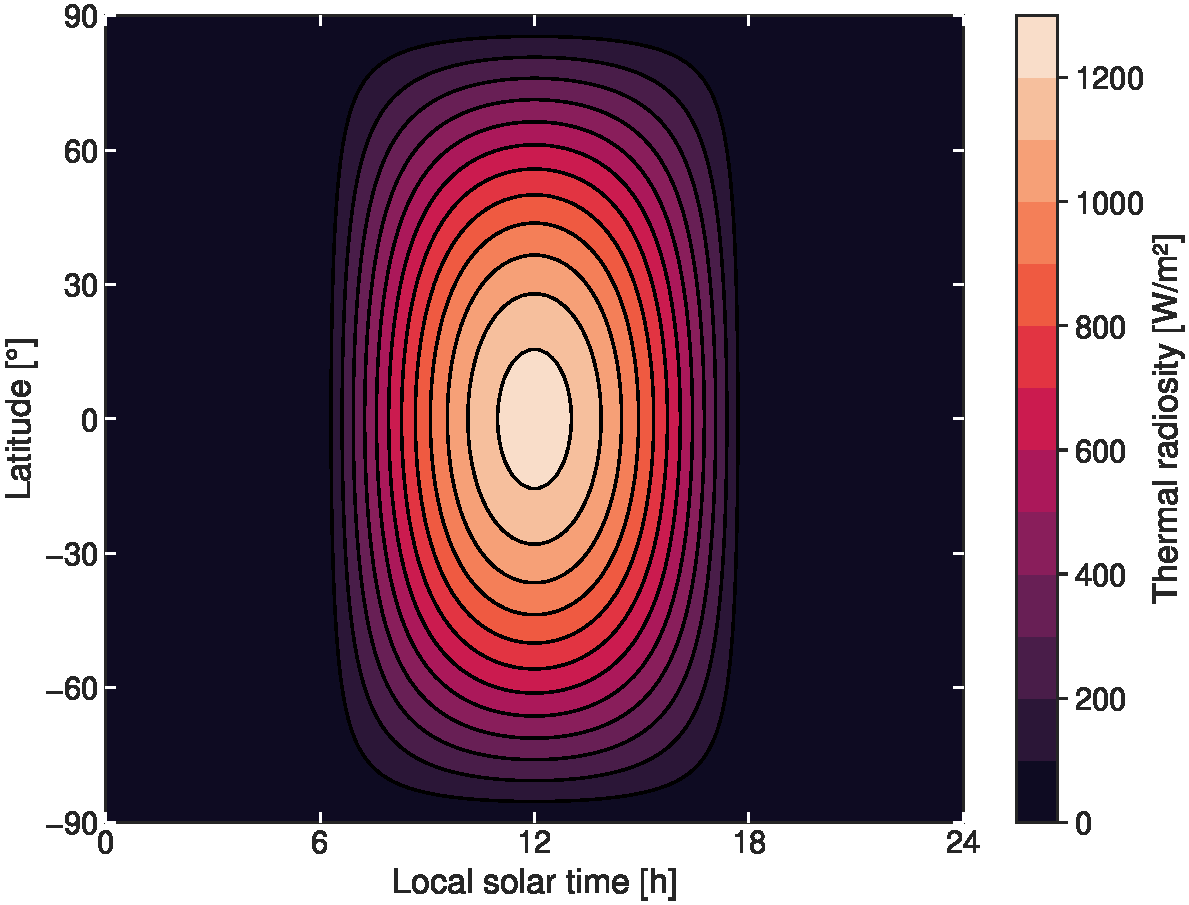
\includegraphics[width=\linewidth]{figures/plots/thermal_map.pdf}
    \caption{Map of lunar thermal emissions from the angle-based model (\cref{eq:radiosity-thermal-anglebased}). The emissivity is 0.95 and surface temperatures range between \qty{95}{\K} and \qty{385}{\K}, depending on the subsolar angle.}
    \label{fig:thermal-map}
\end{figure}

The thermal surface radiosity $J_\textnormal{thermal}$ from the angle-based model with the aforementioned parameters is shown in \cref{fig:thermal-map}. The radiosity decreases with the cosine of the incidence angle and approaches negligible emissions of \qty{6}{\irr} at nighttime. The maximum radiosity, which occurs below the subsolar point (i.e., at local noon), is \qty{1246}{\irr}. This peak value agrees with those used to design \gls{LRO}'s thermal control subsystem~\cite{Tooley2010}. The only effect that is not captured is the slow cooling by about \qty{25}{\K} between sunset and sunrise~\cite{Vasavada2012}, which introduces a slight asymmetry; we use constant pre-sunrise temperatures throughout the night. We also do not model seasonal variations of surface temperature.





\subsection{Paneling of the Moon}

Knocke's dynamic paneling method described in \cref{subsec:radiation-sources} will be used for the Moon. \gls{LRO}'s low altitude compared to the lunar radios prohibits any static paneling, which would have a large number of never-visible panels.

\begin{figure}[t]
    \centering
    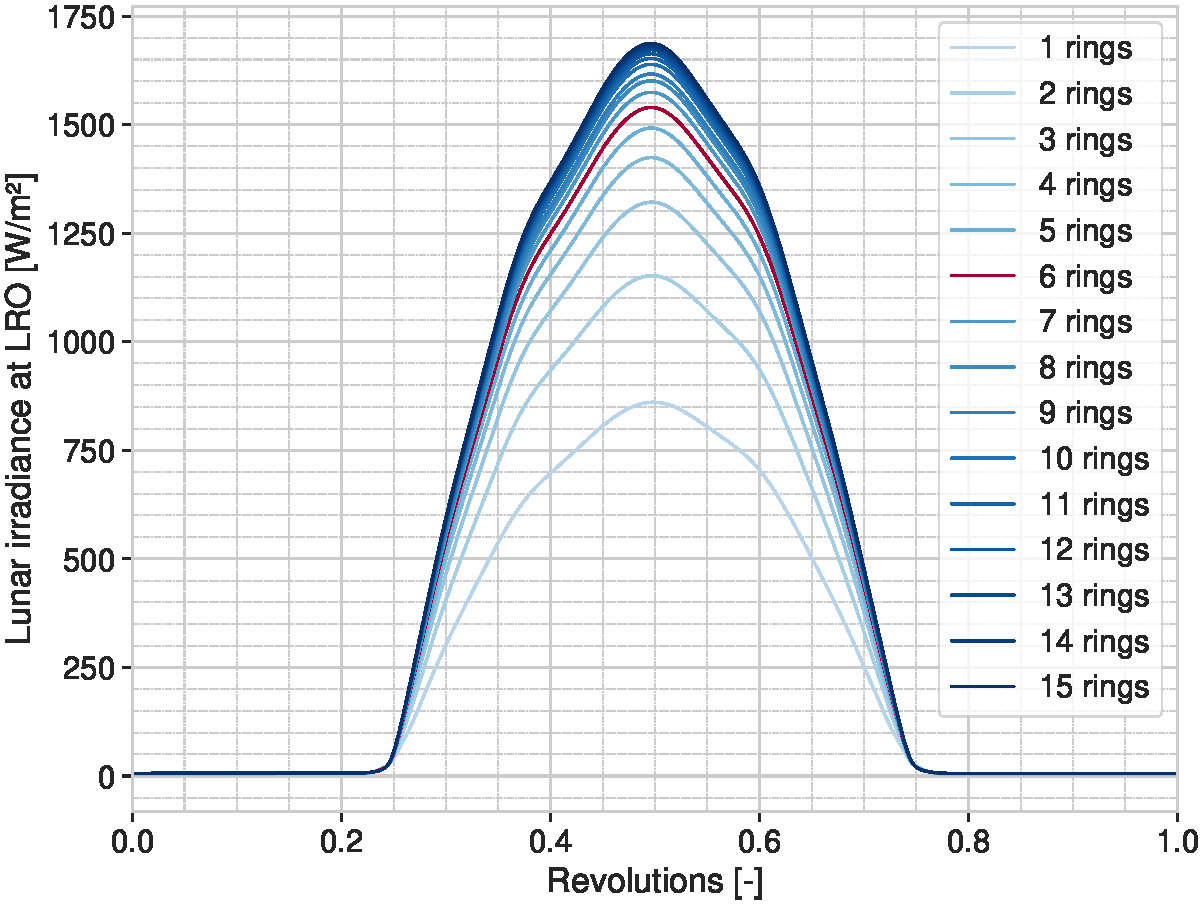
\includegraphics[width=\linewidth]{figures/plots/paneling_convergence.pdf}
    \caption{Convergence of lunar irradiance received by \gls{LRO} for increasing number of rings. Each ring contains six more panels than the previous. Six rings (\textcolor{mpl-red}{\textbf{---}}) are sufficient for an error of less than \qty{10}{\percent} with respect to the converged solution.}
    \label{fig:paneling-convergence}
\end{figure}

Selecting the number of rings is a trade-off between fidelity and computational efficiency. To determine the lowest number of rings that can still represent lunar radiation with sufficient accuracy, we investigated the convergence behavior. \Cref{fig:paneling-convergence} shows the albedo and thermal irradiance received by \gls{LRO} for an increasing number of rings. As suggested by \citeauthor{Knocke1988}, each ring contains six more panels than the previous one. For 13 rings and more, the peak irradiance is within \qty{1}{\percent} of \qty{1687}{\irr}. For six rings, the irradiance peaks at \qty{1540}{\irr}, which is within \qty{10}{\percent} of the converged solution. The results are similar for constant and \gls{DLAM1} albedo.

We choose six rings as sufficiently accurate, which contain 127 panels in total. The panel geometry in this case was already shown in \cref{fig:general-knocke-paneling-low}. This is one ring (or 36 panels) more than used by others. \citeauthor{Floberghagen1999} suggests five rings for Lunar Prospector, which has twice the orbital altitude of \gls{LRO} and thus needs fewer rings (\citeauthor{Knocke1988} only used two rings for a much higher altitude relative to the planetary radios). Five rings are also used for \gls{LRO}'s operational orbit determination~\cite{Nicholson2010}. We choose one ring more to keep the error due to paneling below \qty{10}{\percent}. A higher number may be required in case of a higher-resolution albedo distribution




\subsection{LRO target}

\begin{figure}[t]
    \centering
    \includegraphics[width=\linewidth]{figures/lro_rendering.ai}
    \caption{Rendering of \gls{LRO}~\cite{NSMD2018} including bus frame definition. The X axis is along the velocity vector, the +Y axis is the anti-sun side, and the +Z axis is in the nadir direction~\cite{Tooley2010}.}
    \label{fig:lro-rendering}
\end{figure}

\gls{LRO} consists of a cubical bus with a large solar array and a protruding high gain antenna (\cref{fig:lro-rendering}). The solar array tracks the Sun in two axes, and the antenna points towards Earth whenever it is visible. This leads to large variations in cross-section over time, and different sides are presented to incoming solar and lunar radiation.


\begin{table}[t]
    \centering
    \caption{Panels for \gls{LRO} target model from \citeauthor{Smith2008}~\cite{Smith2008}. The coefficients are for absorptivity and specular/diffuse reflectivity. The solar array is by far the largest surface, followed by the Z-facing panels.}
    \label{tab:target-model}
    \begin{tabular}{lrrrr}
\toprule
\bfseries Panel & \bfseries $\mathbf C_a$ & \bfseries $\mathbf C_s$ & \bfseries $\mathbf C_d$ & $\mathbf A$~[\unit{\meter\squared}] \\
\midrule
\bfseries +X & 0.49 & 0.29 & 0.22 & 2.82 \\
\bfseries -X & 0.42 & 0.39 & 0.19 & 2.82 \\
\bfseries +Y & 0.45 & 0.32 & 0.23 & 3.69 \\
\bfseries -Y & 0.50 & 0.32 & 0.18 & 3.69 \\
\bfseries +Z & 0.50 & 0.32 & 0.18 & 5.14 \\
\bfseries -Z & 0.28 & 0.54 & 0.18 & 5.14 \\
\bfseries +SA & 0.90 & 0.05 & 0.05 & 11.00 \\
\bfseries -SA & 0.50 & 0.30 & 0.20 & 11.00 \\
\bfseries +HGA & 0.54 & 0.18 & 0.28 & 1.00 \\
\bfseries -HGA & 0.93 & 0.02 & 0.05 & 1.00 \\
\bottomrule
\end{tabular}

\end{table}

\gls{LRO} can be modeled as paneled target (\cref{eq:paneled-target}) to account for this variability. The panels are summarized in \cref{tab:target-model}. There are six panels for the bus, with surface normals along the positive and negative axes of the \gls{LRO} bus frame (cf. \cref{fig:lro-rendering}). The solar array and high gain antenna are modeled separately, again with frontside and backside panels. The solar array is almost as large as all other panels combined. Since it always points towards Sun, the solar \gls{RP} will have a large effect. Note that, while tracking of the solar array and antenna are constrained to two axes in reality, we allow three-axis tracking for simplicity. The definitive attitudes of both are also available but were not used since their data volume is prohibitively large. We also neglect self-shadowing, which was shown to only have a minor impact in most cases~\cite{Slojkowski2015,Loecher2018}, but can be significant for solar radiation~\cite{Mazarico2009}.

We also model \gls{LRO} as a cannonball (\cref{eq:cannonball-target}), a model which is often used for orbit determination. Finding a single equivalent cross-section area $A_c$ and \gls{RP} coefficient $C_r$ is virtually impossible~\cite{Vallado2013}. Different values for \gls{LRO} exist in literature: \citeauthor{Bauer2016} use $A_c = \qty{10}{\m\squared}$ and $C_r = 1.2$~\cite{Bauer2016}, while \citeauthor{Nicholson2010} use $A_c=\qty{14}{\m\squared}$ and $C_r = 1.0$~\cite{Nicholson2010}. The acceleration should differ by about \qty{15}{\percent} between them. We choose the latter since it is used for operational orbit estimation of \gls{LRO}.

\begin{figure}[t]
    \centering
    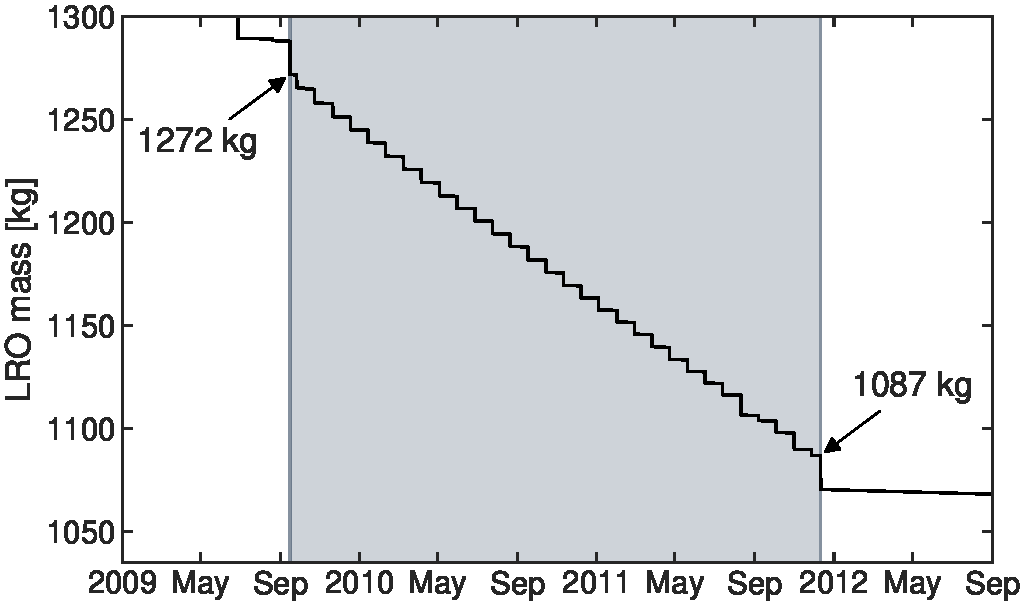
\includegraphics[width=\linewidth]{figures/plots/mass_history.pdf}
    \caption{Mass evolution of \gls{LRO} over the science mission phase (15 September 2009 -- 11 December 2011, \textcolor[RGB]{206, 211, 217}{\ding{110}}). }
    \label{fig:mass-history}
\end{figure}

To complete the target model, the mass is required to convert forces into accelerations. \gls{LRO} performed monthly station keeping maneuvers during its science mission phase, which reduced the initial mass after science orbit insertion from \qty{1272}{kg} to \qty{1087}{kg} (\cref{fig:mass-history}). With every maneuver, \qty{6.3}{kg} of propellant are expelled~\cite{Mesarch2010}. This increases accelerations by \qty{15}{\percent} over the course of 21 months. To facilitate comparison and obtain worst-case results, we will use the end-of-mission mass of \qty{1087}{kg} in this paper, independently of the actual arc.





\subsection{LRO orbit geometry}
% TODO check results quickly if we use both arcs

variation in altitude is in part due to assumption of spherical moon (polar radius is 2.1 km less than equatorial) -> leads to change in lunar RP magnitude over orbit
sun beta over year + eclipse periods

our maximum eclipse time of 48 min agrees with \cite{Tooley2010}

describe beta angle
maybe figure with orbit geometry for simulated arcs

table for dates with beta angle, distance from sun


\subsection{Simulation setup}

simulation setup in table, explanations in text

earth albedo + thermal radiation can be neglected for LRO since it is less than 0.1\% of solar radiation at moon

solar array tracks Sun, HGA tracks Earth~\cite{Tooley2010}
start at start at 26 June 2010 06:00:00
Earth eclipses Sun during this time
Moon does not eclipse Sun (Sun beta angle is about -90 deg, see~\cite{Tooley2010})

lunar eclipses avoided since we cannot represent multiple occultations

effects of neglecting terrain and self shadowing~\cite{Mazarico2018} sec 4.2 and 4.3


Operational LRO OD does not use lunar albedo due to computational demand, but used for offline reprocessing.
Self-shadowing from \citeauthor{Mazarico2009} is used for reprocessing~\cite{Nicholson2010}

arc length 2.5 days, which is also used for LRO orbit determination~\cite{Mazarico2011}
step 5 s, which is also used for LRO orbit determination~\cite{Mazarico2018}

MOON\_PA frame, IAU\_MOON is in worst case 155 m off~\cite{NAIF2020} (Special PCK and FK for Earth and Moon, slide 14)

integrator + propagator params



two arcs, one for beta = 0 and beta = 90
describe why These
\section{Results}

We analyzed the short-term effects of \gls{RP} by examining accelerations and the position at the end of the 2.5-day arc. While the position is ultimately relevant for precise orbit determination, studying the accelerations in different scenarios and along the orbit can explain the cause of position changes. Additionally, the accelerations underscore differences between models of varying complexity.

To compare two accelerations over time, we used the \gls{RMSE}, which is defined as
\begin{align}
    \text{RMSE}(x, y) = \sqrt{\frac{1}{n}\sum_{i=1}^{n}\left(x_i - y_i\right)^2}.
\end{align}
The \gls{RMSE} describes the difference between two scalar time series $x_i, y_i$ and gives more weight to large deviations. These time series can be the magnitude of accelerations or individual components. The \gls{rRMSE} is defined as
\begin{align}
    \text{rRMSE}(x, y) = \sqrt{\frac{\sum_{i=1}^{n}\left(x_i - y_i\right)^2}{\sum_{i=1}^{n} y_i^2}}
\end{align}
and is useful to compare differences across orders of magnitude.

While the simulation evaluates accelerations in a global frame, the effect of accelerations on the orbit is best analyzed in a spacecraft-fixed coordinate system that is aligned with the orbital track. The RSW coordinate system is one such system, defined by the unit vectors~\cite{Vallado2013}
\begin{align}
    \vb R = \frac{\vb r}{\norm{\vb r}}, \quad
    \vb W = \frac{\vb r \times \vb v}{\norm{\vb r \times \vb v}},
    \quad \textrm{and} \quad \vb S = \vb W \times \vb R.
\end{align}
The radial component $\vb R$ is aligned with the planetocentric position vector $\vb r$. The cross-track component $\vb W$ is aligned with the angular momentum vector, or orbit plane normal, and involves the linear velocity $\vb v$. The along-track component $\vb S$ completes the right-handed coordinate system. Note that $\vb S$ is generally not perfectly aligned with the velocity vector, but can be considered so for \gls{LRO}'s approximately circular orbit.





\subsection{Instantaneous reradiation}
\label{subsec:inst-rerad}

First, we investigated the effect of instantaneous reradiation for the paneled target model. This increases the acceleration proportional to each panel's $C_a$ in a direction normal to the panel (cf. \cref{eq:brdf-reaction-specular-diffuse-instrerad}).

\begin{figure}[t]
    \centering
    \begin{subfigure}[c]{\linewidth}
        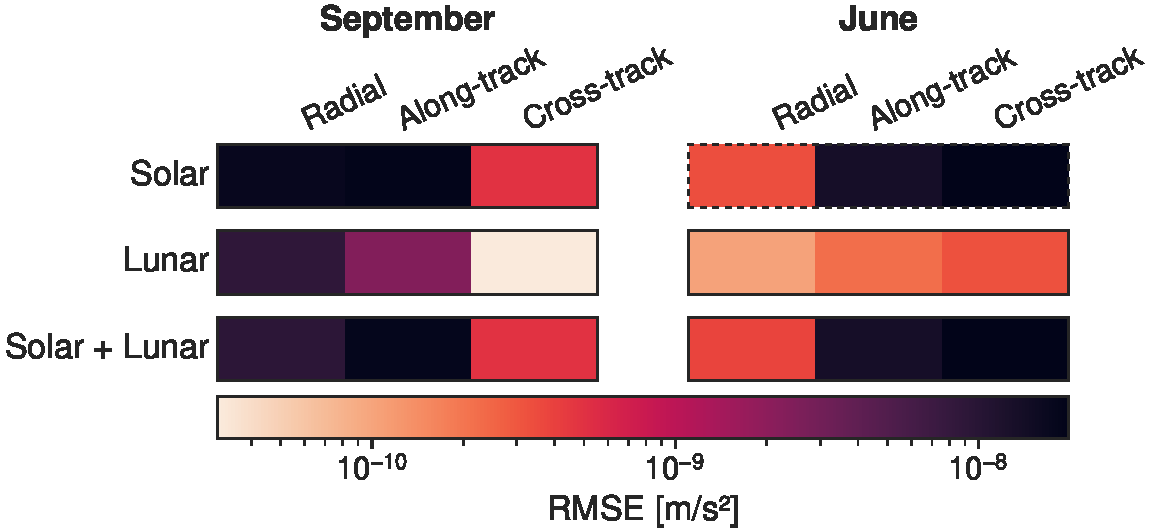
\includegraphics[width=\textwidth]{figures/plots/acc_reradiation_rms.pdf}
        \subcaption{Absolute}
     \end{subfigure}

     \bigskip

     \begin{subfigure}[c]{\linewidth}
        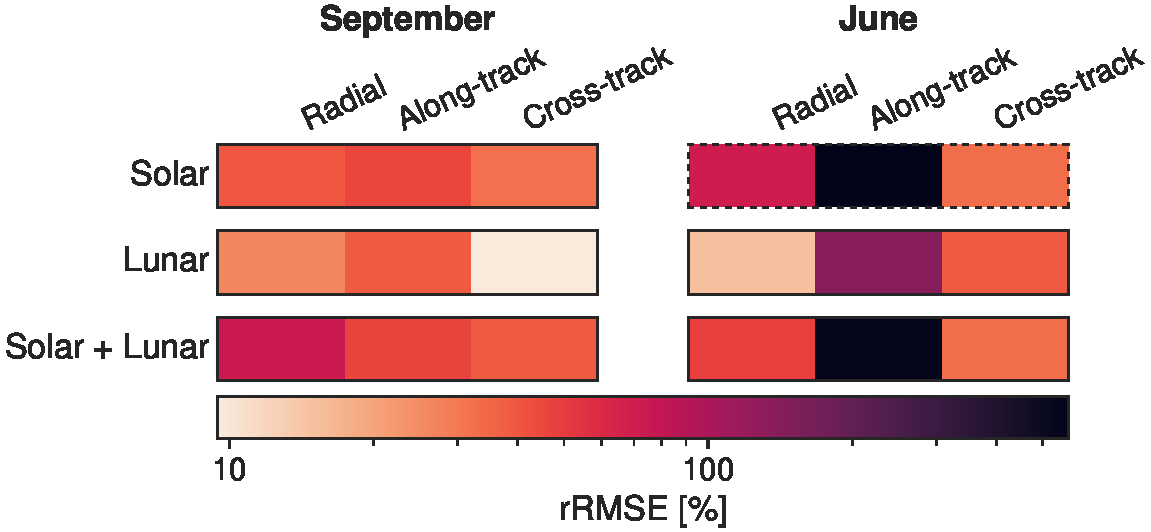
\includegraphics[width=\textwidth]{figures/plots/acc_reradiation_rrms.pdf}
        \subcaption{Relative}
     \end{subfigure}
    \caption{RMS differences of \gls{RP} accelerations over one orbit with and without instantaneous reradiation. The dashed boxes correspond to \cref{fig:acc-reradiation}.}
    \label{fig:acc-reradiation-rms}
\end{figure}

\begin{figure}[t]
    \centering
    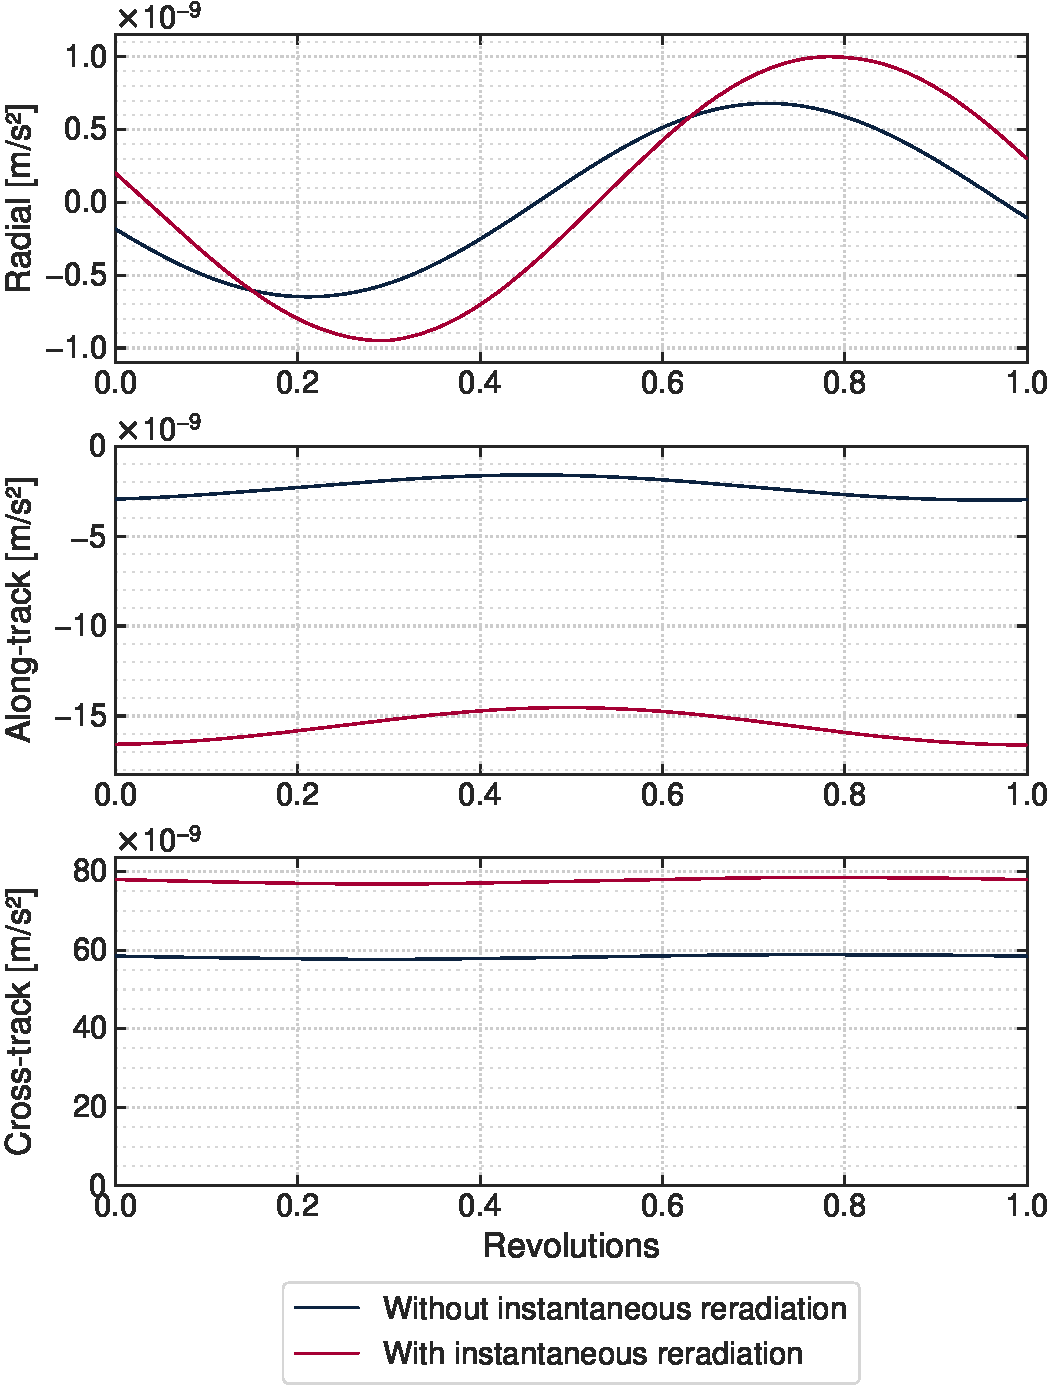
\includegraphics[width=\linewidth]{figures/plots/acc_reradiation_sun_jun.pdf}
    \caption{Accelerations due to solar radiation without and with instantaneous reradiation over one orbit for the June arc. There is a phase shift in the radial component and the along-track component increased by \qty{570}{\percent} \gls{RMSE}. Lunar contributions and the September arc are not significantly affected in shape.}
    \label{fig:acc-reradiation}
\end{figure}

\Cref{fig:acc-reradiation-rms} shows the absolute and relative differences between accelerations without and with instantaneous reradiation. In absolute terms, the radial and along-track components are impacted most for the September arc, while the along-track and cross-track components experience the largest increase for the June arc (for both arcs, up to about \qty{1.9e-8}{\acc} \gls{RMSE}). The relative differences are more uniform (around \qty{40}{\percent} \gls{rRMSE}), but the along-track components of lunar and solar radiation in the June arc increase by \qty{140}{\percent} and \qty{570}{\percent} \gls{rRMSE}, respectively. In most cases, only the magnitude of accelerations changes but not the pattern over an orbit.

\Cref{fig:acc-reradiation} shows the solar radiation of the June arc without and with instantaneous reradiation, the only of our simulations for which the pattern changed significantly. The phase of the radial acceleration is shifted by about \qty{10}{\percent} of the orbital period, which is not the case for the other two components or the acceleration due to lunar radiation. The solar acceleration of the June arc also had the largest relative change in along-track component as described above (highlighted in \cref{fig:acc-reradiation-rms}). This change manifests as a constant offset of about \qty{-13e-9}{\acc}. 

The large changes seen in some cases are mostly due to the +SA panel, which is highly absorptive ($C_a = 0.90$) and large ($A = \qty{11.00}{\m\squared}$). For the June arc, the solar array is angled at \qty{45}{\degree} with equal components in the cross-track and along-track directions The Sun is on the same side as the solar array in the cross-track direction. Without instantaneous reradiation, no panel has a significant contribution to the along-track acceleration, so it is quite small at around \qty{2e-9}{\acc}. With instantaneous reradiation, each panel, and especially the solar array, exerts an acceleration parallel to its normal, which leads to the along-track increase witnessed for the June arc.

We applied instantaneous reradiation for all of the following simulations since no reradiation due to spacecraft panels is physically unrealistic and the differences in magnitude are significant when instantaneous reradiation is added. More sophisticated thermal models involving conduction and internal heat generation would likely produce more accurate results.




% \subsection{Simulation setups}

% Solar with/without
% Lunar with/without
% Albedo none/constant/dlam
% Thermal none/angle-based
% LRO cannonball/paneled
% with/without isntantaneous reradiation
% Beta angle/arc

% 46 simulations





\subsection{Accelerations}
\label{subsec:results-accelerations}

The most direct effect of \gls{RP} is visible in the accelerations. Therefore, we compare the \gls{RP} accelerations
\begin{itemize}
    \item for the September and June arcs,
    \item due to solar and lunar (albedo + thermal) radiation,
    \item for the constant and \gls{DLAM1} albedo distributions,
    \item for the cannonball and paneled targets.
\end{itemize}
In total, we ran 46 simulations. All accelerations are given in \qty{e-9}{\acc}. Regarding the cannonball and paneled target models, note that their comparative magnitudes are less important since the choice of cannonball parameters is somewhat arbitrary. Instead, we compared their behaviors and how they relate to model assumptions (e.g., symmetry for the cannonball, tracking for the paneled target).


\subsubsection{Solar and lunar radiation}
Both solar and lunar radiation are significant but their accelerations may amplify or cancel each other. To compare them, we used a constant albedo model in addition to the thermal model. The accelerations over one orbit are shown in \cref{fig:acc-solarvslunar}. Note that secular variations in orbit geometry can change the magnitude of acceleration components across orbits even within one 2.5-day arc; secular variations are not shown here.

\begin{figure*}[tb]
    \centering
    \begin{subfigure}[c]{\textwidth}
        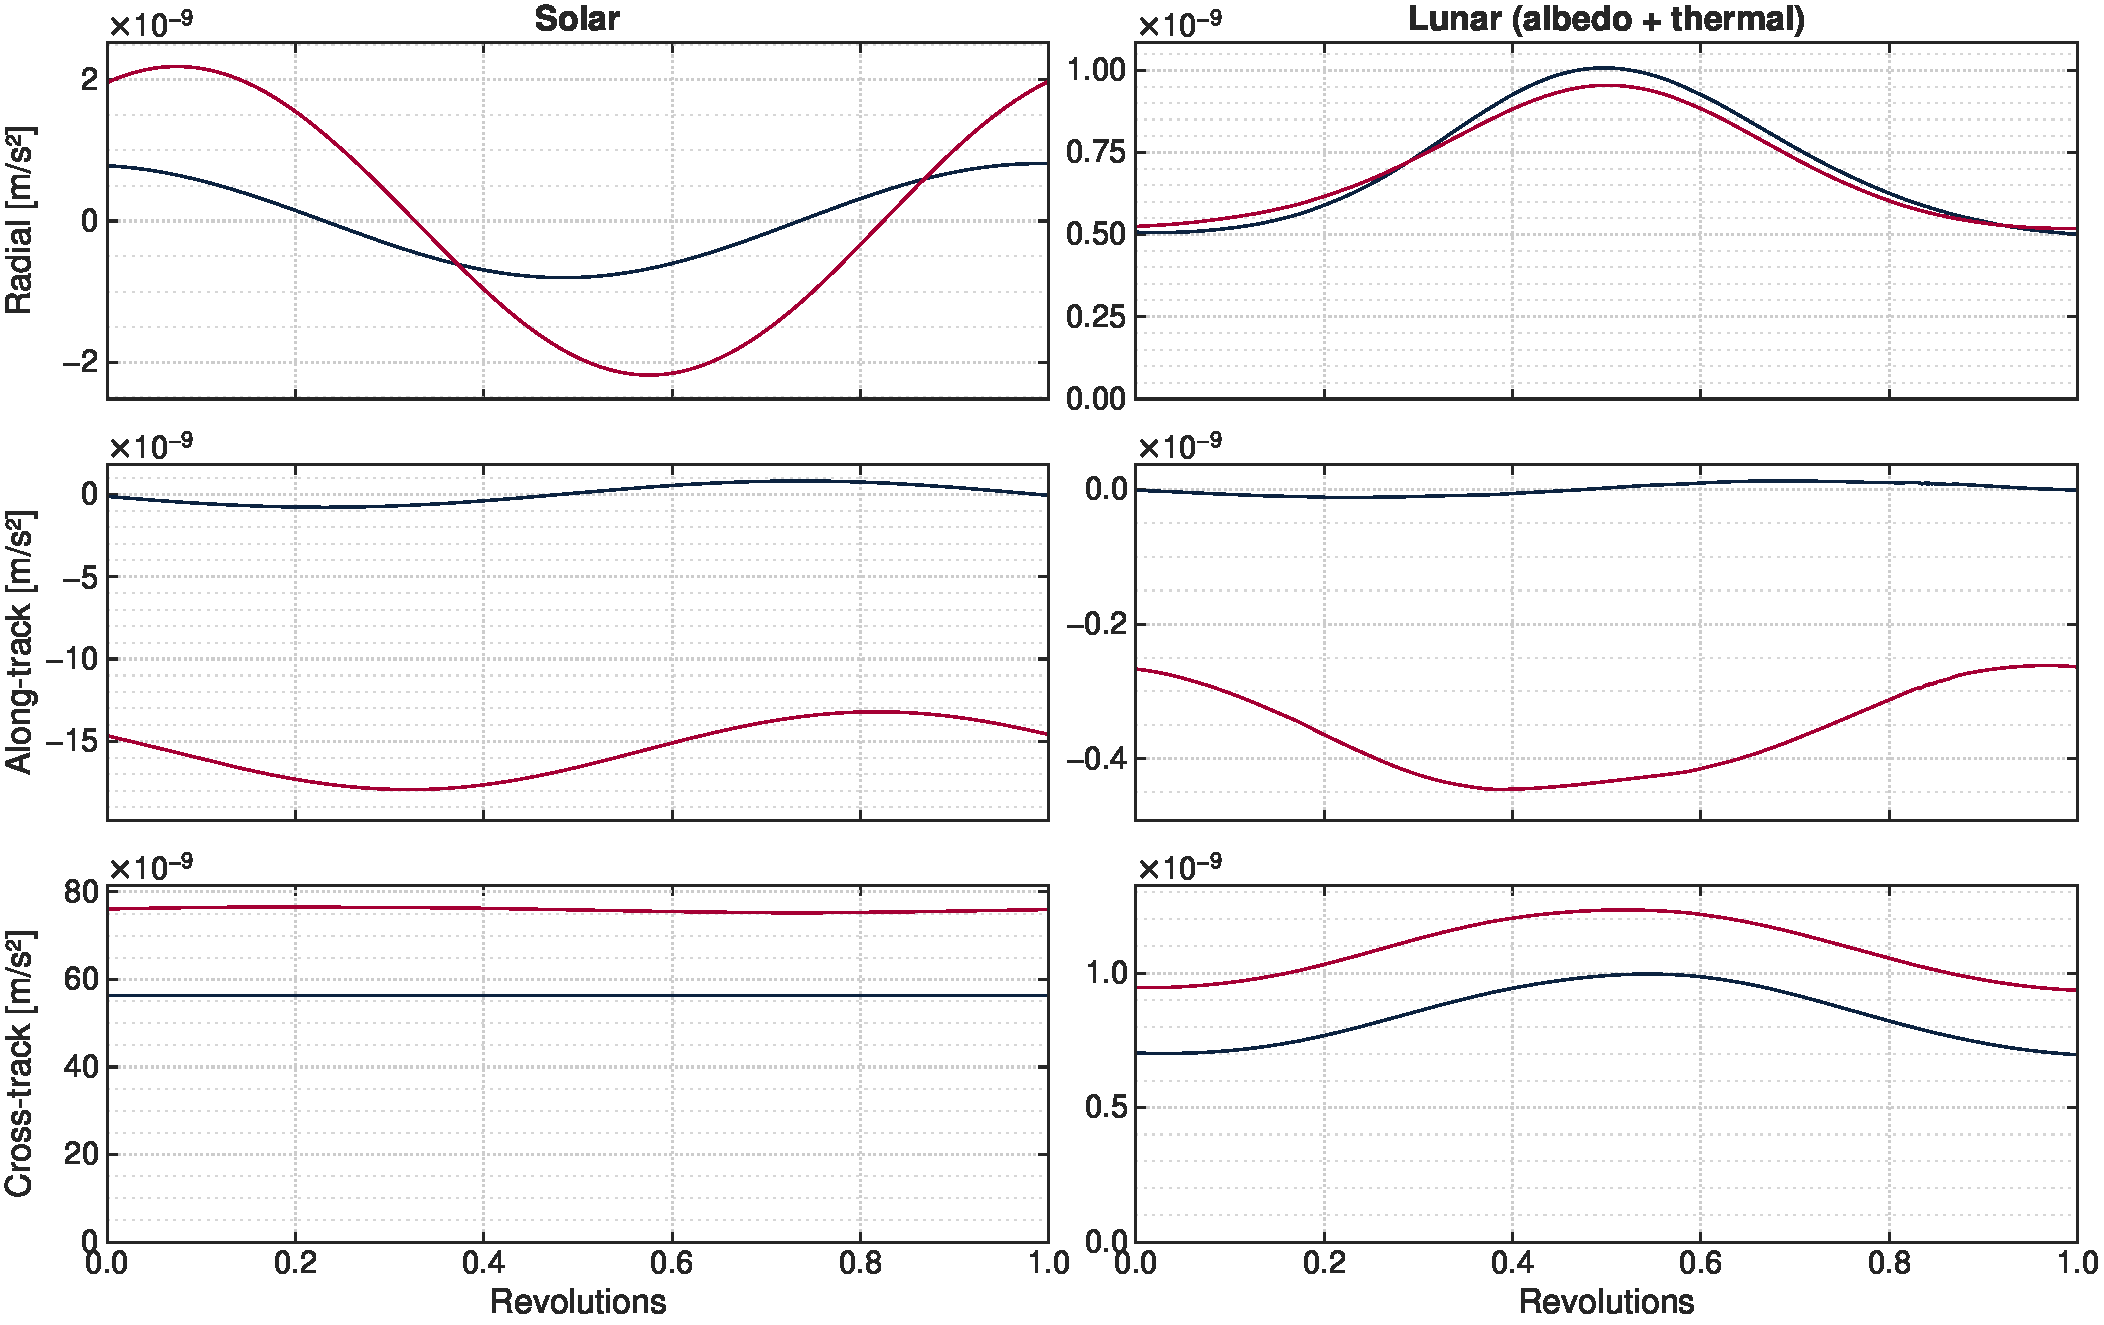
\includegraphics[width=\textwidth]{figures/plots/acc_solarvslunar_jun.pdf}
        \subcaption{June}
        \label{fig:acc-solarvslunar-jun}
     \end{subfigure}

     \bigskip

     \begin{subfigure}[c]{\textwidth}
        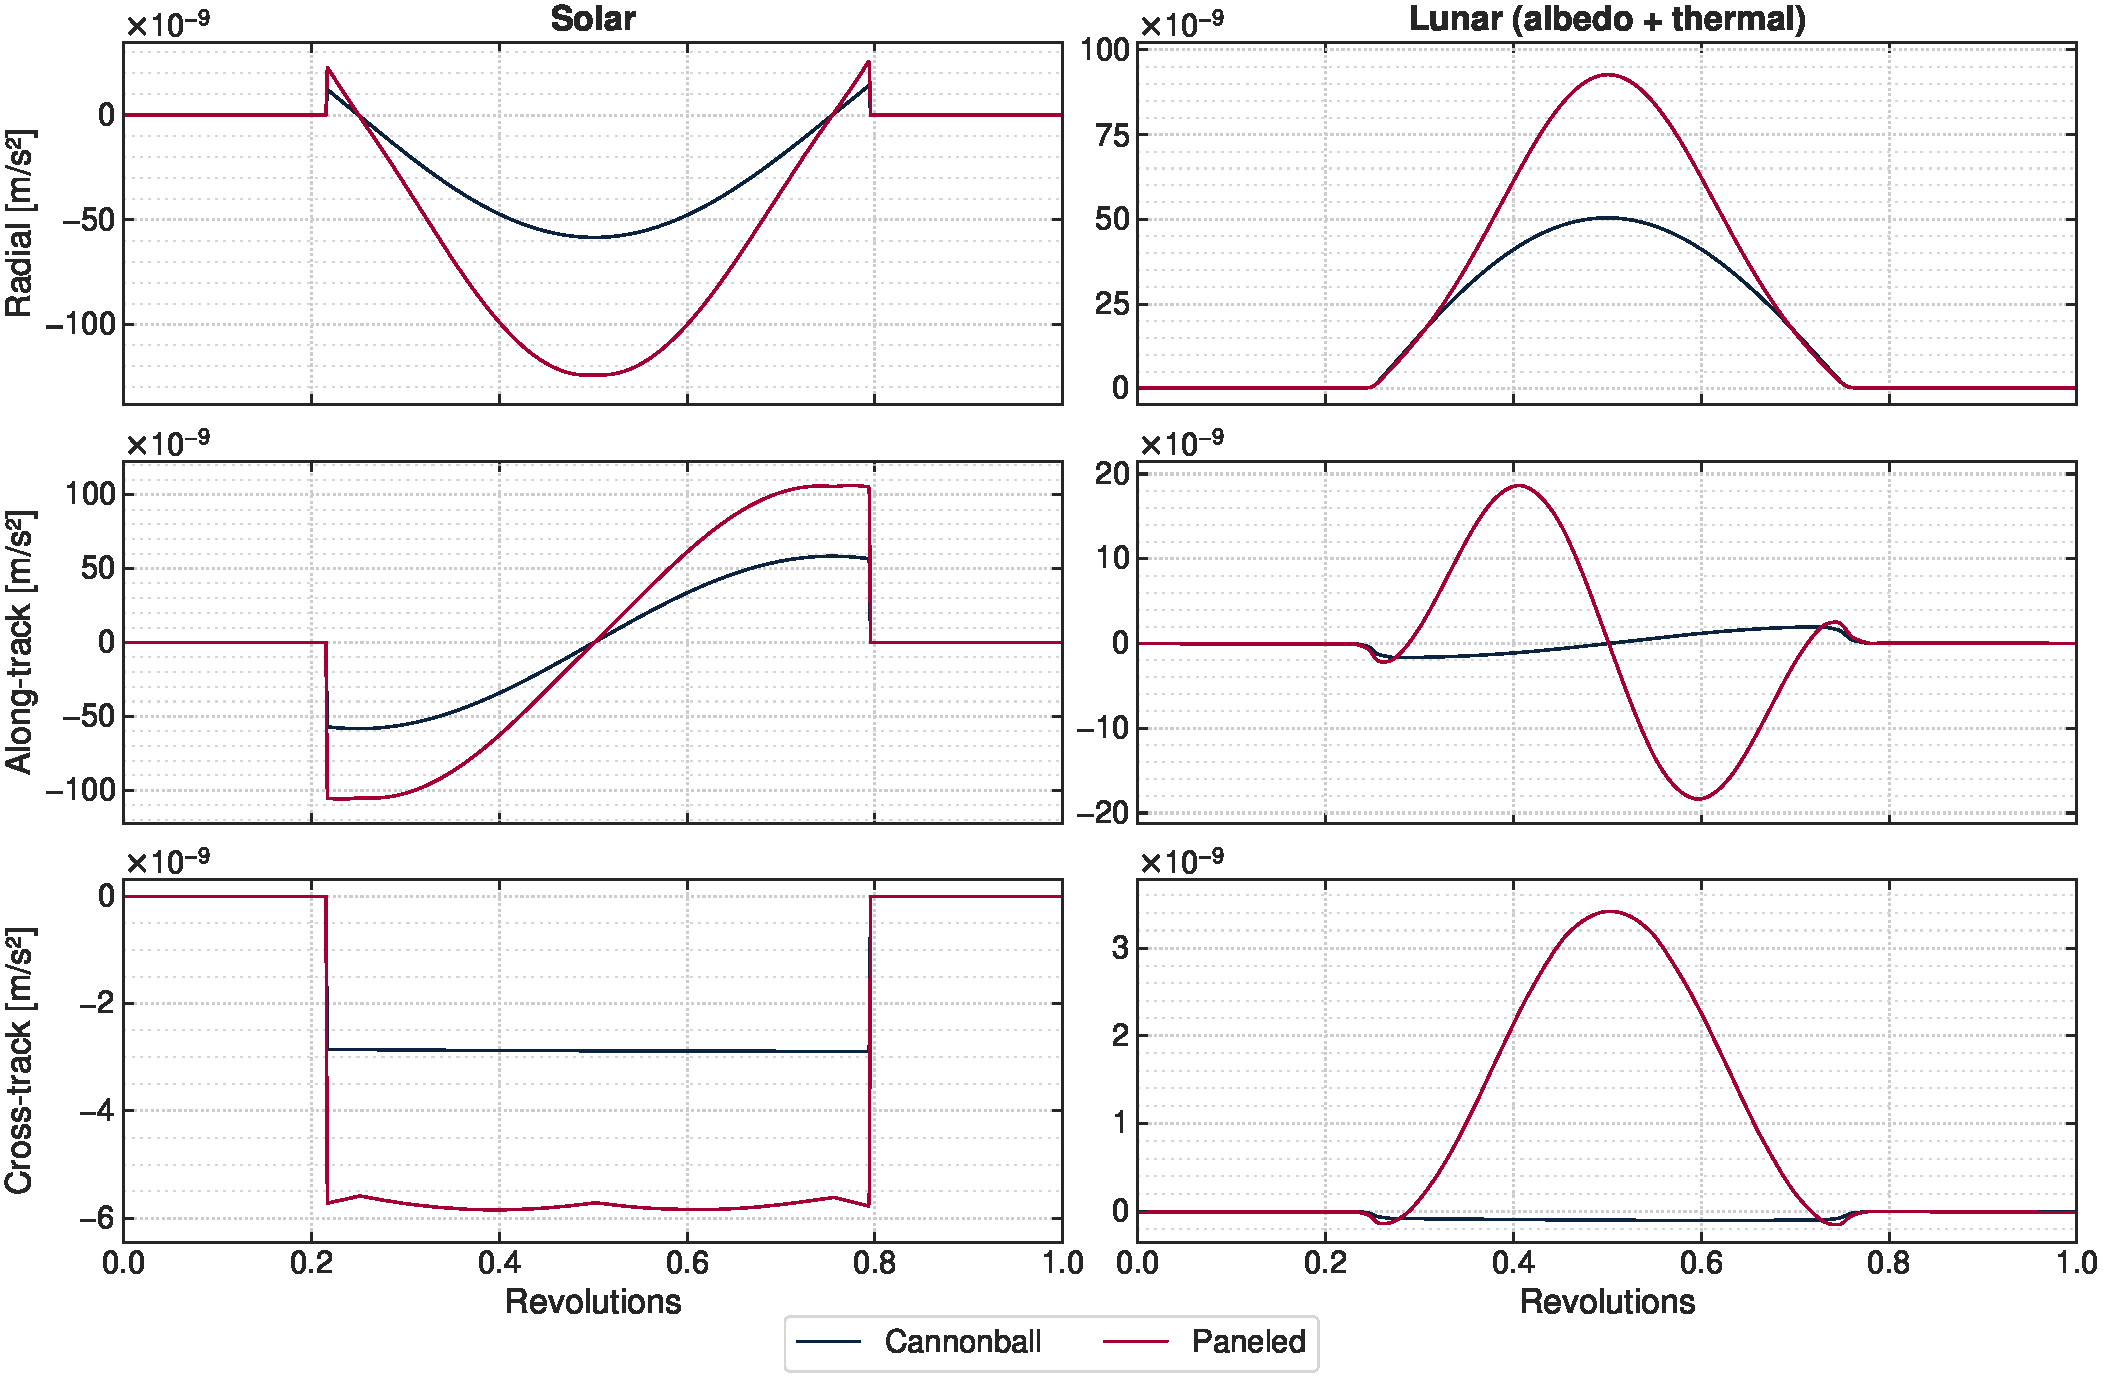
\includegraphics[width=\textwidth]{figures/plots/acc_solarvslunar_sep.pdf}
        \subcaption{September}
        \label{fig:acc-solarvslunar-sep}
     \end{subfigure}

    \caption{Accelerations due to solar and lunar (thermal + constant albedo) radiation over one orbit. The cannonball and paneled targets differ both in magnitude and pattern of accelerations. Note the different scales of each subplot.}
    \label{fig:acc-solarvslunar}
\end{figure*}

For the June arc (\cref{fig:acc-solarvslunar-jun}), the spacecraft is in permanent sunlight and the orbit plane normal points toward the Sun because $\beta \approx \qty{90}{\degree}$. This leads to extremely large, constant cross-track solar accelerations. The paneled model also has along-track solar accelerations due to the solar array as explained in \cref{subsec:inst-rerad}. Interestingly, the radial solar accelerations show the same phase shift between the cannonball and paneled targets as observed without instantaneous reradiation (\cref{subsec:inst-rerad}). This suggests that symmetry, or the lack thereof, is the cause of the phase shift. The magnitude of the total solar acceleration does not change much throughout the year since it is only dependent on the Moon--Sun distance, which is relatively constant at \qty{1}{\astronomicalunit} (see \cref{tab:orbit-geometry}).

The lunar accelerations during the June arc are generally small (less than \qty{2}{\percent} of solar) because \gls{LRO} never passes over well-illuminated regions; half of the lunar source panels that are visible by \gls{LRO} are on the nightside and therefore rarely contribute. The sinusoidal variations in lunar radiation pressure are mainly caused by the fact that $\beta$ is not exactly \qty{90}{\degree} and \gls{LRO}'s angle to the subsolar point therefore varies by \qty{2}{\degree}. Periodic variations in altitude due to the eccentricity itself have a minimal effect since higher altitudes mean larger distances but also a larger visible area of the lunar surface, which roughly cancels. Secular variations in lunar accelerations (not shown) exist and are due to the evolution of eccentricity over the 2.5 days caused by the non-uniform lunar gravity field~\cite{Tooley2010}. The eccentricity ranges from 0.005 to 0.008, which leads to periselene altitudes between \qty{37}{\km} and \qty{41}{\km}. Such changes in eccentricity lead to larger amplitudes but no mean shift.

For the September arc (\cref{fig:acc-solarvslunar-sep}), the Sun is occulted for \qty{42}{\percent} of the orbit since $\beta \approx \qty{0}{\degree}$. The effect of these occultations is evident in solar and lunar radiation, both of which vanish on the nightside. The accelerations are mostly in the radial and along-track directions. This is most clearly explained by the solar accelerations: At $t=\num{0.2}$, \gls{LRO} crosses the terminator above the pole and is moving straight toward the Sun; the along-track component is then maximal and negative since the Sun opposes the spacecraft's motion. Continuing the orbit, \gls{LRO} passes above the subsolar point at $t=\num{0.5}$, leading to a maximal and negative radial component while the along-track component has vanished. Further toward the other pole, \gls{LRO} passes into the night at $t=\num{0.8}$, where the along-track component accelerates the spacecraft into the direction of motion. During this whole time, the cross-track component is slightly negative because $\beta$ is slightly negative but not zero. If $\beta$ were slightly positive, the cross-track component would be similar but with the sign flipped. In addition to periodic changes, there is a secular change in solar accelerations (not shown) since the already slightly negative $\beta$ continues to decrease: over the 2.5-day arc, the mean of the along-track and cross-track components increase twofold and threefold, respectively. This trend continues until the cross-track component dominates for high $\beta$, as seen for the June arc.

The lunar accelerations during the September arc are much larger than during the June arc because \gls{LRO} passes right over the subsolar point, which reflects much sunlight and has high thermal emissions. Indeed, the lunar irradiance (up to \qty{1830}{\irr}) is larger than the solar irradiance (up to \qty{1360}{\irr}) above the subsolar point. Still, the lunar acceleration magnitude is \qty{14}{\percent} smaller than the solar acceleration magnitude since lunar panels are distributed azimuthally around the nadir and thus partially cancel while all solar rays are parallel and therefore compound. Another feature of lunar accelerations is the sign opposite to solar accelerations: when passing over the subsolar point, the radial components of solar and lunar accelerations roughly cancel. A similar effect can be seen in the along-track and cross-track components for a paneled target, although the lunar radiation needs some time to build up: The along-track component peaks at a subsolar angle of \qty{33}{\degree}, the cross-track component above the subsolar point. The cross-track component increases secularly over the 2.5-day arc, similarly to solar radiation.

Comparing the accelerations of cannonball and paneled targets for both arcs, it is clear that a single $C_r$ cannot capture the complex and changing spacecraft geometry. While the solar accelerations for the September arc are just off by about a constant factor, this is not the case for the June arc or any of the lunar accelerations. In fact, the sign may even be different, particularly for lunar along-track and cross-track accelerations in September. This is likely caused by the solar array tracking the Sun. On smaller scales, the effect of target panels of different sizes and reflective properties becoming illuminated as \gls{LRO} revolves around the Moon can be seen in the kinks of the solar cross-track accelerations of the September arc.

All accelerations are inversely proportional to the spacecraft's mass. While we chose the end-of-mission mass for all simulations, the begin-of-mission mass is \qty{17}{\percent} higher and all accelerations are thus \qty{15}{\percent} lower (see \cref{subsec:lro-target}). This only changes magnitudes, not patterns.





\subsubsection{Lunar albedo and thermal radiation}
In the previous subsection, lunar radiation was regarded as the sum of albedo and thermal radiation. In this subsection, we look at the separate contributions and the differences between albedo distributions. The accelerations on a paneled target are shown in \cref{fig:acc-albedovsthermal}.

\begin{figure*}[tb]
    \centering
    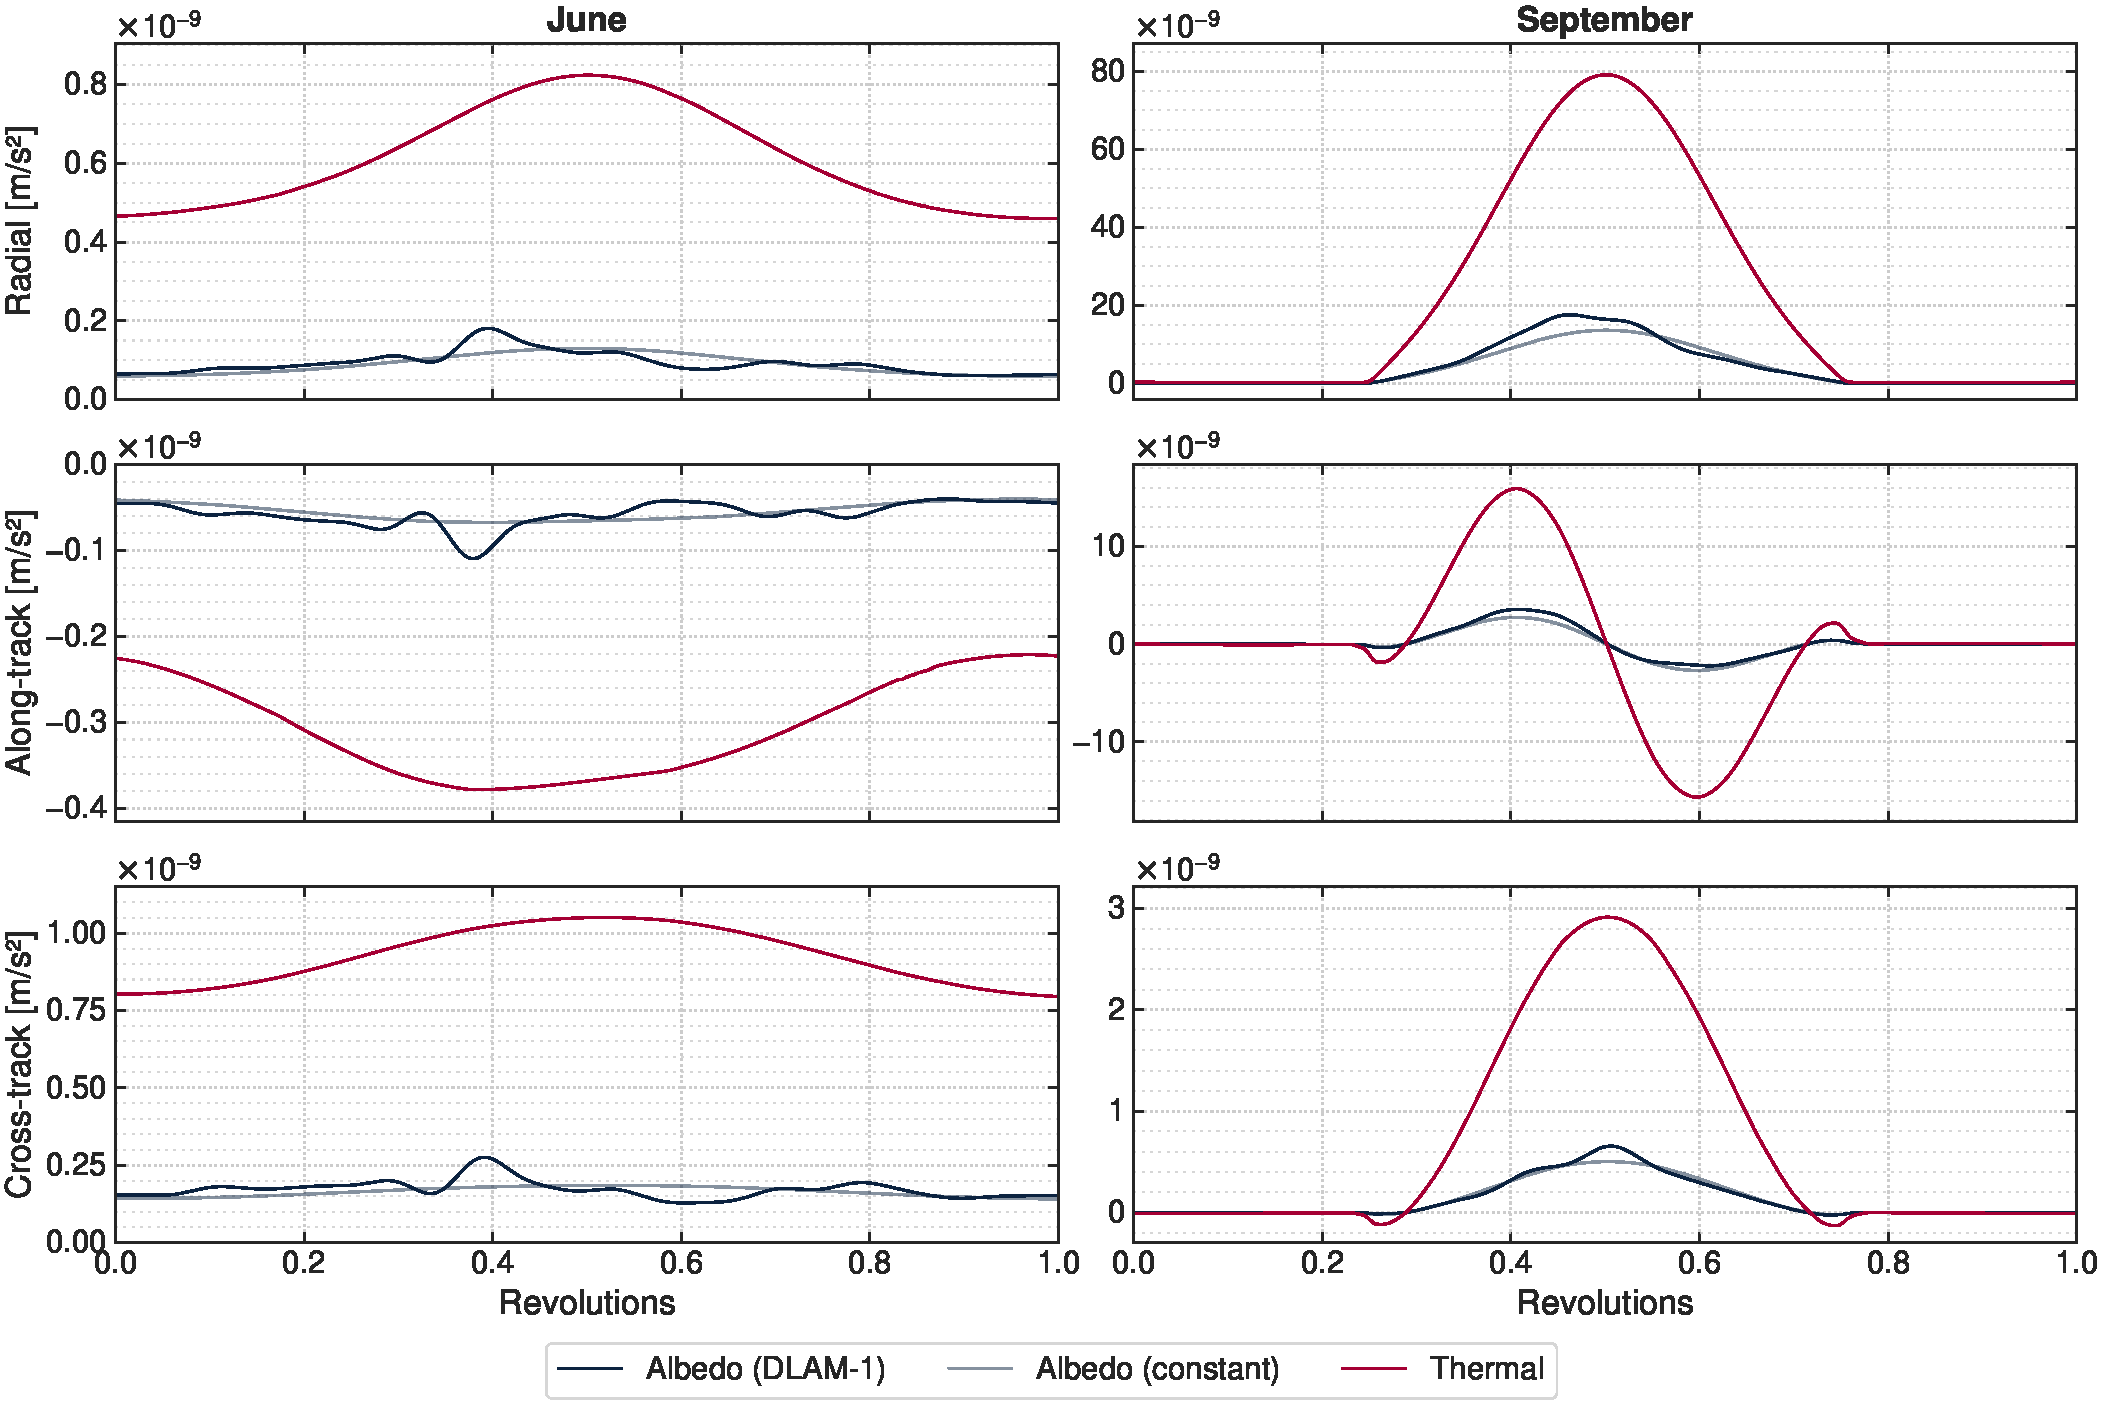
\includegraphics[width=\textwidth]{figures/plots/acc_albedovsthermal.pdf}

    \caption{Accelerations due to lunar thermal and albedo radiation on a paneled target. Thermal radiation dominates at all times and the difference between constant and \gls{DLAM1} albedo is small. Note the different scales of each subplot.}
    \label{fig:acc-albedovsthermal}
\end{figure*}

For both arcs and all components, thermal radiation is far larger than albedo radiation (up to sixfold). This is even though the albedo is likely overestimated by \qty{25}{\percent} as described in \cref{subsec:lunar-albedo}. In terms of behavior, the thermal radiation and constant albedo radiation are very similar: smooth and dependent on the subsolar angle. However, albedo radiation vanishes in the eclipse region of the September arc. The thermal irradiance at \gls{LRO} on the nightside is \qty{6}{\irr}, which leads to a small total acceleration of \qty{1e-9}{\acc}.


\begin{figure}[htb]
    \centering
    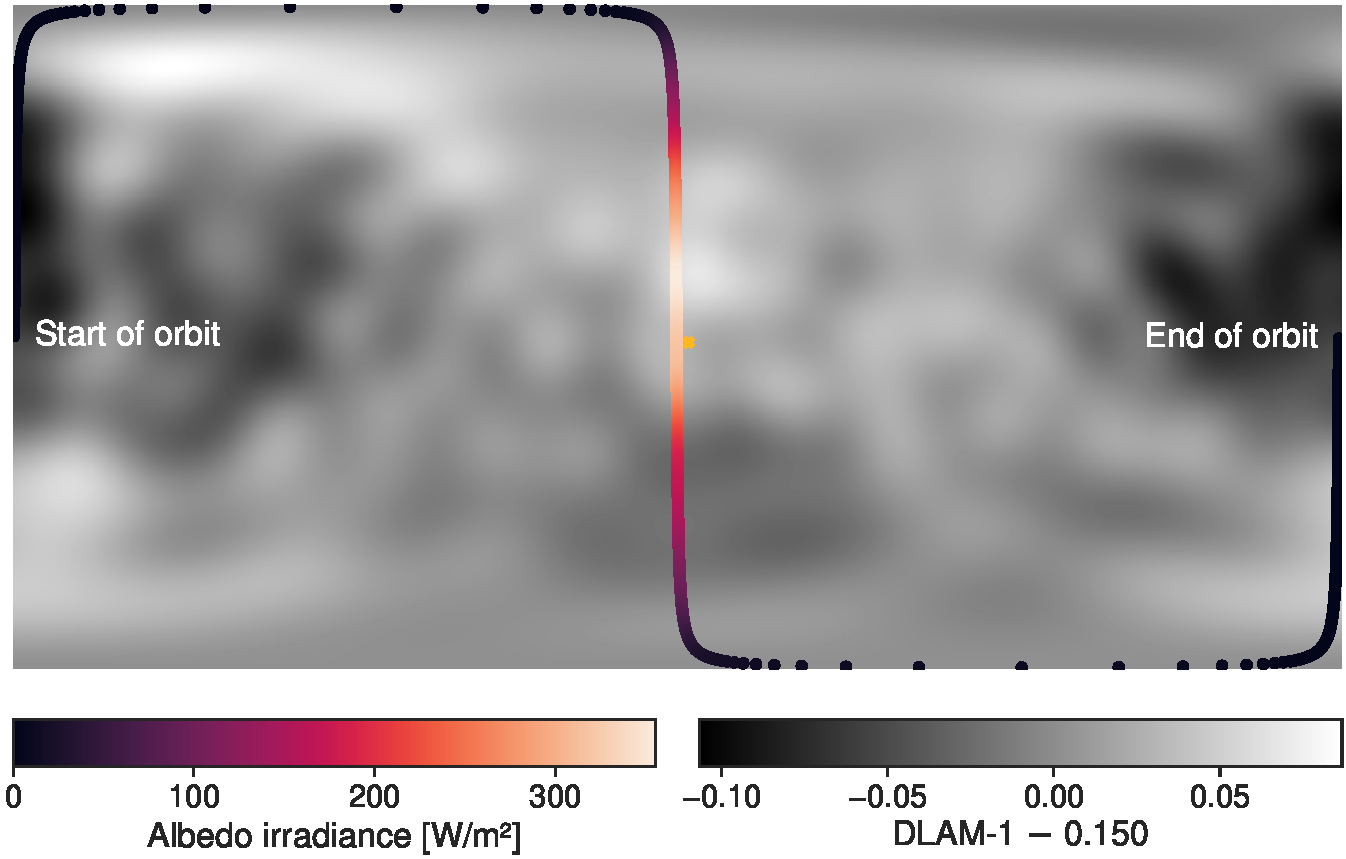
\includegraphics[width=\linewidth]{figures/plots/groundtrack.pdf}
    \caption{Ground track for September arc, colored by the irradiance due to \gls{DLAM1} albedo. The map shows the difference between \gls{DLAM1} and the constant albedo ($a=0.150$). The maximum irradiance does not occur above the subsolar point (\textcolor{mpl-yellow}{\ding{54}}) but above the local albedo maximum \ang{12} north of it.}
    \label{fig:groundtrack}
\end{figure}

The accelerations of the constant and \gls{DLAM1} albedo distributions are of very similar magnitude (in non-zero regions, rRMSE of \qty{14}{\percent} for June and \qty{16}{\percent} for September), although \gls{DLAM1} exihibits irregular variations. The largest difference of \qty{3.7e-9}{\acc} occurs in the radial component for the September arc at $t \approx \num{0.45}$. Interestingly, \gls{DLAM1} albedo radiation peaks \emph{before} the subsolar point, whereas the thermal and constant albedo radiation peak above it. This behavior can be explained by \cref{fig:groundtrack}, which shows the \gls{DLAM1} albedo irradiance along the ground track over a map of the difference between \gls{DLAM1} and the constant albedo. In this figure, the maximum albedo difference also appears before the subsolar point in a region where \gls{DLAM1} has an albedo that is \num{0.043} higher or \qty{29}{\percent} more reflective than the constant albedo of $a=0.150$. All irregular differences between the albedo distributions seen in \cref{fig:acc-albedovsthermal} are explained by this map. Note that larger differences than those seen in June and September may occur for other arcs. However, because the thermal radiation is so much larger, the effect of these differences remains overall limited. Therefore, a constant albedo may be sufficient for most applications.








\subsection{Change in final position}
The goal of orbit determination is to estimate the state, and particularly the position, of a spacecraft over time. Therefore, the difference in position at the end of the arc between models is highly relevant. As mentioned in \cref{sec:introduction}, the maximum allowable error for \gls{LRO} is \qtyrange{50}{100}{\m} in total position and below \qty{1}{\m} radially. Since the true position is not known and this paper is rather concerned with relative differences, we used a simulation without solar and lunar radiation as a baseline reference.

\begin{table*}[tb]
    \caption{Difference of final position in \unit{\m} with respect to the no-\gls{RP} baseline, given as mean over the final orbit plus/minus periodic variations around that mean. The largest changes are in the along-track position. $\mathbf{A}$: solar only; $\mathbf{B}$: lunar only (thermal + constant albedo); $\mathbf{C}$: lunar only (thermal + \gls{DLAM1} albedo); $\mathbf{D}$: solar + lunar (thermal + \gls{DLAM1} albedo).}
    \label{tab:final-position}
    \begin{subtable}[c]{\textwidth}
        \begin{tabular}{llllllllll}
\toprule
 & \multicolumn{4}{c}{\bfseries Cannonball} & \bfseries  & \multicolumn{4}{c}{\bfseries Paneled} \\
 & Radial & Along-track & Cross-track & RMSE &  & Radial & Along-track & Cross-track & RMSE \\
\cmidrule{2-5}\cmidrule{7-10}
\bfseries A & $\num{+0.0 \pm 0.2}$ & $\num{-0.5 \pm 0.5}$ & $\num{+0.1 \pm 0.1}$ & $\num{0.6}$ & ~ & $\num{-7.5 \pm 6.7}$ & $\num{+1066.1 \pm 39.3}$ & $\num{+0.1 \pm 0.2}$ & $\num{1033.5}$ \\
\bfseries B & $\num{+0.0 \pm 0.0}$ & $\num{-0.3 \pm 0.0}$ & $\num{+0.0 \pm 0.0}$ & $\num{0.3}$ & ~ & $\num{-0.2 \pm 0.2}$ & $\num{+24.4 \pm 0.9}$ & $\num{+0.0 \pm 0.0}$ & $\num{23.6}$ \\
\bfseries C & $\num{+0.0 \pm 0.0}$ & $\num{-0.3 \pm 0.0}$ & $\num{+0.0 \pm 0.0}$ & $\num{0.3}$ & ~ & $\num{-0.2 \pm 0.2}$ & $\num{+24.6 \pm 0.9}$ & $\num{+0.0 \pm 0.0}$ & $\num{23.9}$ \\
\bfseries D & $\num{+0.0 \pm 0.2}$ & $\num{-0.8 \pm 0.4}$ & $\num{+0.1 \pm 0.1}$ & $\num{0.8}$ & ~ & $\num{-7.7 \pm 6.9}$ & $\num{+1090.7 \pm 40.2}$ & $\num{+0.1 \pm 0.2}$ & $\num{1057.4}$ \\
\bottomrule
\end{tabular}

        \subcaption{June}
     \end{subtable}

     \medskip

     \begin{subtable}[c]{\textwidth}
        \begin{tabular}{llllllllll}
\toprule
 & \multicolumn{4}{c}{\bfseries Cannonball} & \bfseries  & \multicolumn{4}{c}{\bfseries Paneled} \\
 & Total & Radial & Along & Cross &  & Total & Radial & Along & Cross \\
\cmidrule{2-5}\cmidrule{7-10}
\bfseries Solar only & $60.9_{-24.9}^{+23.9}$ & $0.2_{-12.1}^{+12.4}$ & $-36.4_{-25.1}^{+23.8}$ & $0.0_{-0.4}^{+0.5}$ & ~ & $108.3_{-48.1}^{+45.1}$ & $0.3_{-23.0}^{+23.7}$ & $-61.8_{-47.7}^{+45.6}$ & $0.0_{-0.9}^{+0.9}$ \\
\bfseries Lunar only (constant) & $7.4_{-5.4}^{+5.8}$ & $0.1_{-2.9}^{+2.8}$ & $-12.2_{-5.9}^{+5.2}$ & $0.0_{-0.1}^{+0.1}$ & ~ & $2.4_{-11.6}^{+11.2}$ & $0.1_{-6.1}^{+5.9}$ & $-11.6_{-12.4}^{+11.4}$ & $0.0_{-0.2}^{+0.2}$ \\
\bfseries Lunar only (DLAM-1) & $7.7_{-5.5}^{+5.9}$ & $0.1_{-2.9}^{+2.8}$ & $-12.6_{-6.0}^{+5.3}$ & $0.0_{-0.1}^{+0.1}$ & ~ & $10.8_{-11.8}^{+12.5}$ & $0.1_{-6.2}^{+6.1}$ & $-21.4_{-12.9}^{+11.3}$ & $0.0_{-0.2}^{+0.2}$ \\
\bfseries Solar + lunar (DLAM-1) & $68.4_{-18.2}^{+19.3}$ & $0.2_{-9.2}^{+9.5}$ & $-49.1_{-19.8}^{+17.8}$ & $0.0_{-0.4}^{+0.4}$ & ~ & $118.7_{-33.6}^{+35.4}$ & $0.4_{-17.0}^{+17.5}$ & $-83.2_{-36.3}^{+32.7}$ & $0.0_{-0.6}^{+0.6}$ \\
\bottomrule
\end{tabular}

        \subcaption{September}
     \end{subtable}
\end{table*}

The differences in final positions with respect to the baseline simulation are shown in \cref{tab:final-position}. The first number is the mean, secular difference over the final orbit (32nd revolution), and the second number gives the amplitude of periodic variations around that mean over the final orbit. Note that the periodic variation is quite large in some cases despite zero secular change.

The June arc shows a large along-track difference (more than \qty{1}{\km}) for the paneled target with solar radiation ($\mathbf{A}$). This is likely due to accumulation of the consistently large along-track acceleration of about \qty{-15e-9}{\acc}. However, this acceleration is of lower magnitude than the constant acceleration of \qty{+47e-9}{\acc} expected to result in this position difference, and of the opposite sign. For the cannonball, the along-track accelerations have a zero mean and thus the position difference is also zero. This, again, reveals how the cannonball cannot account for asymmetry; with symmetric accelerations, no secular changes occur. Interestingly, the large cross-track acceleration does not lead to a large cross-track difference in the final position. Positions with constant and \gls{DLAM1} albedo ($\mathbf{B}$ and $\mathbf{C}$) do not differ significantly.

For the September arc, the cannonball and paneled targets give more similar results. Again, the largest secular difference is in the along-track position. However, in contrast to the June arc, \gls{LRO} is shifted back in the track this time. Due to the large variations in radial and along-track accelerations over each orbit, there are large periodic variations in the radial and along-track positions too. For the paneled target with solar and lunar radiation ($\mathbf{D}$), these have amplitudes of \qty{18}{\m} and \qty{36}{\m} for the radial and along-track differences, respectively. The periodic variations have higher amplitudes when not including lunar radiation ($\mathbf{A}$), which otherwise cancel solar accelerations partially (see \cref{subsec:results-accelerations}). There also is a \qty{7}{m} RMSE difference for the paneled model in September between constant and \gls{DLAM1} albedo, the only of the four cases where the choice of albedo model influences the final position.


These differences in position emphasize the importance of \gls{RP} models for precise orbit determination. The best approximation of the true effect of \gls{RP} is given by setup $\mathbf{D}$ (solar + lunar radiation) with a the paneled target. For both arcs, the maximum allowable total error would be exceeded by the superposition of secular and periodic variations if \gls{RP} were neglected. The radial requirement of sub-meter accuracy would be violated by periodic variations alone.




% \subsection{Change in orbital element}

% No good results since Tudat calculates elements from propagation frame, not Moon frame

% \begin{landscape}
    
%     \begin{table}
%         \small
%         \caption{Difference of Kepler elements with respect to no-\gls{RP} baseline, given as mean over the final orbit. The elements are the semi-major axis ($a$ in \unit{m}), eccentricity ($e$, unitless), inclination ($i$ in \unit{\degree}), longitude of the ascending node ($\Omega$ in \unit{\degree}), and argument of periapsis ($\omega$ in \unit{\degree}).}
%         \label{tab:final-elements}
%         \begin{subtable}[c]{\textwidth}
%             \begin{tabular}{llllllllllll}
\toprule
 & \multicolumn{5}{c}{\bfseries Cannonball} & \bfseries  & \multicolumn{5}{c}{\bfseries Paneled} \\
 & $a$ & $e$ & $i$ & $\Omega$ & $\omega$ &  & $a$ & $e$ & $i$ & $\Omega$ & $\omega$ \\
\cmidrule{2-6}\cmidrule{8-12}
\bfseries Solar only & \num{+0.0015} & \num{+8.3e-10} & \num{+1.2e-06} & \num{-1.8e-06} & \num{+0.001} & ~ & \num{-7.2} & \num{-2.6e-07} & \num{+7.1e-06} & \num{+5.3e-06} & \num{+0.0022} \\
\bfseries Lunar only (constant) & \num{+7.4e-05} & \num{+5.7e-10} & \num{-1.2e-07} & \num{+1.8e-07} & \num{-7.2e-05} & ~ & \num{-0.17} & \num{-8.6e-09} & \num{+8.8e-08} & \num{+3.9e-07} & \num{-4.8e-05} \\
\bfseries Lunar only (DLAM-1) & \num{+7.6e-06} & \num{-1.9e-10} & \num{-6.4e-08} & \num{+2.1e-07} & \num{-7.3e-05} & ~ & \num{-0.17} & \num{-9.4e-09} & \num{+1.6e-07} & \num{+4.2e-07} & \num{-4.1e-05} \\
\bfseries Solar + lunar (DLAM-1) & \num{+0.0015} & \num{+6.4e-10} & \num{+1.2e-06} & \num{-1.6e-06} & \num{+0.00097} & ~ & \num{-7.4} & \num{-2.7e-07} & \num{+7.2e-06} & \num{+5.7e-06} & \num{+0.0021} \\
\bottomrule
\end{tabular}

%             \subcaption{June}
%          \end{subtable}
    
%          \medskip
    
%          \begin{subtable}[c]{\textwidth}
%             \begin{tabular}{llllllllllll}
\toprule
 & \multicolumn{5}{c}{\bfseries Cannonball} & \bfseries  & \multicolumn{5}{c}{\bfseries Paneled} \\
 & $a$ & $e$ & $i$ & $\Omega$ & $\omega$ &  & $a$ & $e$ & $i$ & $\Omega$ & $\omega$ \\
\cmidrule{2-6}\cmidrule{8-12}
\bfseries Solar only & \num{+0.23} & \num{-5.8e-06} & \num{+5.7e-06} & \num{+1.3e-05} & \num{-0.027} & ~ & \num{+0.4} & \num{-1.1e-05} & \num{+1.1e-05} & \num{+2.6e-05} & \num{-0.052} \\
\bfseries Lunar only (constant) & \num{+0.039} & \num{+1.3e-06} & \num{+1.4e-07} & \num{-3.1e-06} & \num{+0.0062} & ~ & \num{+0.039} & \num{+2.8e-06} & \num{-4.1e-06} & \num{-6.5e-06} & \num{+0.013} \\
\bfseries Lunar only (DLAM-1) & \num{+0.041} & \num{+1.3e-06} & \num{+1.6e-07} & \num{-3.1e-06} & \num{+0.0061} & ~ & \num{+0.1} & \num{+2.8e-06} & \num{-4.3e-06} & \num{-6.6e-06} & \num{+0.013} \\
\bfseries Solar + lunar (DLAM-1) & \num{+0.27} & \num{-4.4e-06} & \num{+5.8e-06} & \num{+1e-05} & \num{-0.021} & ~ & \num{+0.5} & \num{-8.2e-06} & \num{+6.6e-06} & \num{+1.9e-05} & \num{-0.038} \\
\bottomrule
\end{tabular}

%             \subcaption{September}
%          \end{subtable}
%     \end{table}

% \end{landscape}

% compare wih Gauss perturbing equations (analytical solution to change of osculating elements based on accelerations), e.g. ~\cite[Sec.~3.2]{Lucchesi2006}

% Keplerian state wrt ECLIPJ2000, not Moon frame!!

% prediction september: change in arg peri because solar along-track acts fully above poles without being cancelled by lunar rad

% for september: sign of change of inclination and lon asc node depends on sign of beta




\subsection{Performance}
Choosing the appropriate model is not only a consideration of accuracy but also one of computational effort. The aim is to find the most efficient model that is sufficiently accurate. To determine how much less efficient complex models like paneled targets or \gls{DLAM1} are, we measured wall time durations for different model combinations. We ran each simulation 100 times in random order on a server with 2 Intel Xeon E5-2683 v3 CPUs (14 cores each, two threads per core with hyperthreading) while no other loads were present. 27 simulations ran in parallel such that all but one core were used. More parallelism would have triggered hyperthreading, which would have skewed measurements. \gls{Tudat} was compiled in release configuration with GCC 7.5.0 at optimization level \texttt{-O2}. No other steps such as CPU pinning were taken. Note that software performance can be influenced by many, seemingly innocuous aspects~\cite{Mytkowicz2009}. Still, the results show the general tendency.

\begin{figure}[b]
    \centering
    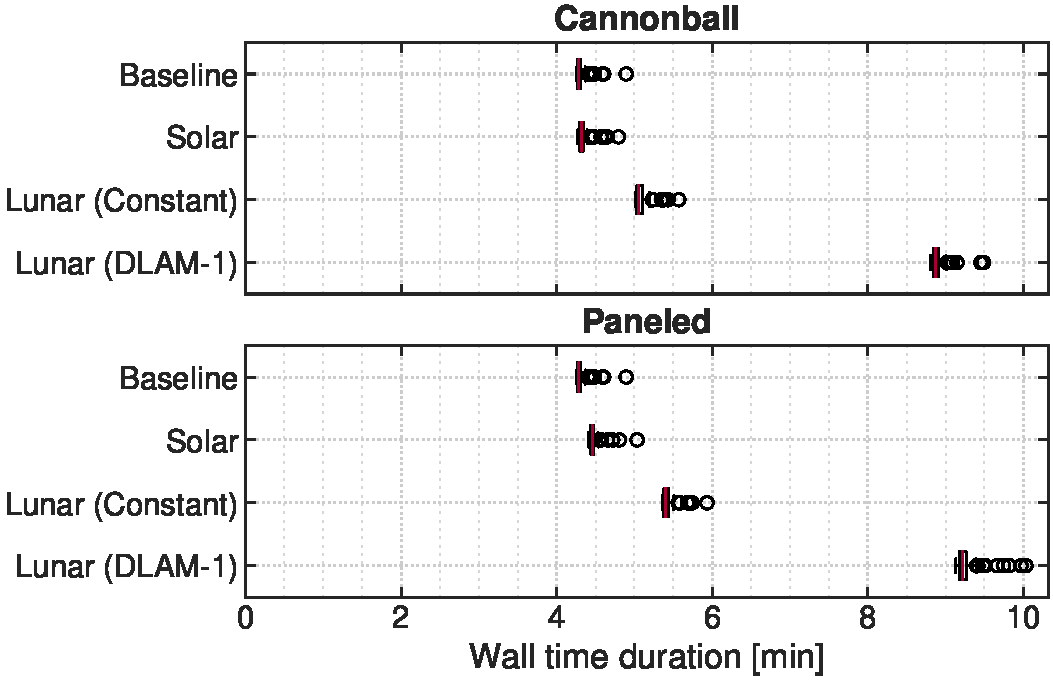
\includegraphics[width=\linewidth]{figures/plots/performance.pdf}
    \caption{Wall time duration of simulations with different \gls{RP} models. The statistics come from 100 runs for each model. Evaluation of \gls{DLAM1}'s spherical harmonics expansion increases the duration by up to \qty{80}{\percent}.}
    \label{fig:performance}
\end{figure}

The wall time durations when including solar or lunar radiation are shown in \cref{fig:performance}. Again, the baseline simulation without radiation serves as a reference. The median baseline time of \qty{4.3}{\min} includes computations for general integration and propagation, the lunar spherical harmonics gravity model, and point gravities from Sun and Earth. Solar radiation has a negligible complexity, even for a paneled target. Lunar radiation with constant albedo increases the duration by about \qty{20}{\percent}, but slightly more for the paneled than the cannonball target. These values depend highly on the number of source panels. The spherical harmonics expansion of \gls{DLAM1} is computationally expensive and increases the duration by up to \qty{80}{\percent} compared to the baseline. This is a significant performance penalty, which may not always be tolerable. Other authors even report increases of several hundred percent for \gls{DLAM1} albedo~\cite{Nicholson2010}.

The durations are relatively consistent as indicated by the inter-quartile range of at most \qty{5}{\s}. Still, all distributions have a long tail toward longer durations: the difference between maximum and median is between 9 and 21 times higher than the difference between minimum and median. This skewness is typical for software performance.

\section{Conclusion}

We described a collection of \gls{RP} models of varying levels of complexity, then examined the differences in short-term orbital effects of \gls{RP} on \gls{LRO} between these models. There are large seasonal differences in the \gls{RP} accelerations: for small $\beta$ (e.g., around September), the accelerations are mainly radial and along-track, while they are predominantly cross-track for $\beta \approx \pm \ang{90}$ (e.g., around June). After 2.5 days, the position diverged from the no-\gls{RP} baseline by up to \qty{1100}{\m} in June and \qty{80}{\m} in September. Periodic variations of up to \qty{50}{\m} are superimposed over the orbit on the secular differences. In September, the periodic variations are damped by lunar accelerations that oppose solar accelerations. Large differences also exist between the representations of \gls{LRO} as a cannonball and a paneled target: due to the cannonball's symmetry, accelerations do not cancel over an orbit and are generally smaller than those of a paneled target, which can have the solar array track the Sun. Thermal radiation dominates the lunar emissions, and a constant albedo distribution is both sufficiently accurate and computationally cheaper than the spherical harmonics expansion \gls{DLAM1}.

Our results showed that \gls{RP} is essential for precise orbit determination of the \gls{LRO}. Both the total and radial accuracy requirements would be violated otherwise. However, not all models are worth the computational effort. We recommend the following setup:
\begin{itemize}
    \item Solar radiation should be included since it is significant yet computationally cheap.
    \item Lunar thermal and constant albedo radiation should be included since it only increases walltime duration by \qty{20}{\percent} and affects secular and periodic variations significantly. To reduce the performance impact, fewer rings could be used, although the lunar irradiance will then be underestimated.
    \item The spatial variations in albedo from \gls{DLAM1} do not increase the accuracy much despite the performance penalty of \qty{80}{\percent}. Therefore, it should not be included unless the utmost accuracy is desired (particularly in September). The spherical harmonics expansion could also be truncated to improve performance.
    \item The paneled target should be included since the cannonball underestimates accelerations and does not account for Sun tracking of the solar array. The performance impact of the paneled target is negligible.
    \item The cannonball target should only be included if its coefficient is estimated since a constant coefficient cannot represent changes in geometry and orientation. Even then, consistent estimation of the coefficient is difficult at small $\beta$~\cite{Slojkowski2014}.
\end{itemize}

While we restricted our investigation to a small number of models, the short-term orbital effect of these more involved models should also be investigated:
\begin{itemize}
    \item Self-shadowing, particularly for solar radiation, can reduce the effective cross-section by up to \qty{40}{\percent} for large $\beta$~\cite{Mazarico2018}.
    \item Moon topography can advance eclipse onset by up to \qty{480}{\s} for $\beta > \ang{70}$~\cite{Mazarico2018}. The conical shadow model should be replaced by one that evaluates lines of sight based on topography.
    \item \gls{DLAM1} was published in 1999 based on miscalibrated Clementine imagery, which overestimates the actual albedo. A new spherical harmonics model should be fitted from more recent, properly calibrated imagery.
    \item Accelerations due to thermal reradiation by the spacecraft itself can be significant. Our model of instantaneous reradiation should be replaced by one that accounts for heating and conduction.
    \item The lunar opposition effect increases albedo radiation for low phase angles much more than Lambertian reflectance predicts. Such phase angles occur for small $\beta$. The Hapke \gls{BRDF} with spatially resolved parameter maps~\cite{Sato2014} should be used for albedo reflection.
    \item Post-sunset lunar thermal radiation is underestimated because gradual cooling to nighttime temperatures is not reflected in our thermal model. It should be replaced with a more physical model due to the large magnitude of thermal compared to albedo radiation.
\end{itemize}



\FloatBarrier



\begin{codeav}
The code is available at \url{https://github.com/DominikStiller/tudelft-hpb-project}.
\end{codeav}


\printbibliography

\end{document}
